\documentclass[10pt]{amsbook}

\usepackage{mathtools}
\usepackage{hyperref}
\usepackage{amsmath}
\usepackage{amsthm}
\usepackage{algorithm}
\usepackage{algpseudocode}
\usepackage{listings}
\usepackage{tikz}
\usepackage{fancybox}
\usepackage{tablefootnote}
\usepackage{float}

\floatstyle{boxed}
\restylefloat{figure}

\newtheorem{theorem}{Theorem}[section]
\newtheorem{exmp}{Example}[section]

\begin{document}
\title{SpliceMachine Architecture}
\author{Scott Fines}

\maketitle
\begingroup
\let\clearpage\relax
\chapter*{Introduction}
SpliceMachine is a next generation HTAP data management platform.  They system is designed from the ground up to address 3 challenging pieces of the distributed data management landscape.

Transactions: Splice Machine provides a transactional system that can support both OLAP and OLTP transactions.  Analytical systems require transactional capabilities around bulk imports, index maintenance, and consistent scans of multiple data sources.  OLTP systems require transactions for critical business process execution.

Analytical Execution:

Transactional Execution:




\endgroup

\tableofcontents
\begingroup
\let\clearpage\relax
\chapter{Transactions}
\section{Transactional Structure}
It is useful to take some time and define transactions cleanly, so that future conversations can use consistent notation and terminology.

Loosely speaking, a transaction is a sequence of events that appears to be single-threaded to the end user, even if there are multiple such transactions concurrently modifying the same data.

More precisely, we choose a \emph{begin timestamp} $T_b$ and a \emph{commit timestamp} $T_c$ to be positive numbers such that $T_c >T_b$ (e.g. the commit timestamp must \emph{always} come after the begin timestamp). Then, we define a \emph{transaction} $T$ to be the interval $[T_b,T_c)$ such that all event which occur between $T_b$ and $T_c$ are viewed sequentially.

Of course, "Sequentially" gets us into some trouble here, but to be clear, let us consider two transactions $T_1 = [T_{b1},T_{c1})$ and $T_2 = [T_{b2},T_{c2})$. We have the following possibilities:

\begin{enumerate}
				\item $T_{c1} < T_{b2}$. In this case $T_1$ is said to have occurred \emph{before} $T_2$.
				\item $T_{c2} < T_{b1}$. In this case $T_2$ occurs \emph{before} $T_1$.
				\item $T_{b1} < T_{b2} < T_{c1}$. In this case, $T_1$ and $T_2$ are said to be occurring \emph{simultaneously}
\end{enumerate}

Our intuition tells us that, in any "sequential" situation, $T_1$ occuring before $T_2$ implies that any actions taken by $T_1$ should affect $T_2$. In this sense, we say that an action is \emph{visible} to a transaction whenever it can affect the transaction's behavior. So, if $T_1$ occurs before $T_2$, any writes that were made inside of $T_1$ should be visible to $T_2$, in that $T_2$'s queries will be affected by them.

This defines the central rule of transactions: 

\begin{theorem}
				If a transaction $T_1 = [T_{b1},T_{c1})$ occurs before another transaction $T_2 = [T_{b2},T_{c2})$(that is, $T_{c1} < T_{b2}$), then any actions taken by $T_1$ are visible to $T_2$.
\end{theorem}

\begin{exmp}[Transaction Visibility]
				Suppose Alice wishes to write the value "hello" to a row. To do this, she
				\begin{enumerate}
					\item acquires begin timestamp $T_{ba} = 1$
					\item writes data
					\item acquires commit timestamp $T_{ca} = 2$ and finishes her transaction
				\end{enumerate}
				After this is done, Bob wishes to read the same row. To do this, he acquires a begin timestamp $T_{bb} = 3$ and attempts to read the row. Because $T_{ca} < T_{bb}$, Alice's write is visible, so Bob's transaction sees the value "hello".
\end{exmp}

This rule does not illustrate what is to be done when $T_1$ and $T_2$ occur simultaneously; this is an abiguity which cannot be resolved without assistance from the user.

To deal with this ambiguity,we introduce the concept of \emph{isolation levels}. In essence, an isolation level is simply a user-defined rule for how to deal with simultaneous transaction activity.

Consider those same transactions $T_1$ and $T_2$ again, but suppose that they are occurring simultaneously. There are three possible approaches for a user to take:

\begin{description}
				\item[Read Uncommitted] Data is visible to $T_2$ whenever $T_{b1} < T_{c2}$.
				\item[Read Committed] Data is visible to $T_2$ whenever $T_{c1} < T_{c2}$.
				\item[Repeatable Reads] Data is visible to $T_2$ whenever $T_{c1} < T_{b2}$.
\end{description}

These three are defined as the three possible isolation levels\footnote{Sometimes, there is a fourth level: \emph{Serializable}, which deals with how to deal with conflicting write attempts. It is pretty heavily tied to transaction implementations, and as such I leave it out here. }.

\subsection{Read Uncommitted Visibility}
Consider the following example.
\begin{exmp}[Read Uncommitted Visibility]
				Suppose that there is a row containing the content "hello". Alice wishes to modify that data, and Bob wishes to read that data, and both are attempting to operate simultaneously in time. Then the following sequence occurs:
				\begin{enumerate}
					\item Alice acquires begin timestamp $T_{ba} = 1$.
					\item Alice writes "goodbye" to row
					\item Bob acquires begin timestamp $T_{bb} = 2$
					\item Bob reads row. Because $T_{ba} < T_{bb}$ and Bob is using a Read Uncommitted isolation level, Bob is able to see Alice's changes, so he sees the text "goodbye"
					\item Alice acquires commit timestamp $T_{ca} = 3$ and commits her write	
				\end{enumerate}
\end{exmp}
In this case, Bob was able to see Alice's writes,even though Alice had not yet committed, a situation we call \emph{dirty reading}. There are advantages to read uncommitted (usually performance), but it is subject to several transactional anomalies.

First, there is a \emph{false reads} issue. Consider this variation on the above example:

\begin{exmp}[Dirty Read Anomaly]
				Suppose that there is a row containing the content "hello". Alice wishes to modify that data, and Bob wishes to read that data, and both are attempting to operate simultaneously in time. Then the following sequence occurs:
\begin{enumerate}
	\item Alice acquires begin timestamp $T_{ba} = 1$.
	\item Alice writes "goodbye" to row
	\item Bob acquires begin timestamp $T_{bb} = 2$
	\item Bob reads row. Because $T_{ba} < T_{bb}$ and Bob is using a Read Uncommitted isolation level, Bob is able to see Alice's changes, so he sees the text "goodbye"
	\item Alice writes "hello" back to row
	\item Alice acquires commit timestamp $T_{ca} = 3$ and commits her write	
\end{enumerate}
\end{exmp}
At the end of this operation, the row contains data "hello", but Bob acted upon it as if it were "goodbye", potentially causing incorrect results\footnote{This is even more significant when the possibility of rolling back a transaction is introduced}.

Secondly, there is an ordering issue. Notice in the above example that Alice wrote "goodbye" before Bob attempted to read it. However, the following sequence is equally possible:

\begin{exmp}[Operation Ordering anomaly]
				Suppose that there is a row containing the content "hello". Alice wishes to modify that data, and Bob wishes to read that data, and both are attempting to operate simultaneously in time. Then the following sequence occurs:
\begin{enumerate}
	\item Alice acquires begin timestamp $T_{ba} = 1$.
	\item Bob acquires begin timestamp $T_{bb} = 2$
	\item Bob reads row. Because Alice has not yet physically written her data, Bob will see the previous value "hello"
	\item Alice writes "goodbye" to row
	\item Alice acquires commit timestamp $T_{ca} = 3$ and commits her write	
\end{enumerate}
\end{exmp}
So read uncommitted can (and often does) result in nondeterministic results--the physical ordering of writes in the implementation determines the results of the query, even within the same transaction.

\subsection{Read Committed Visibility}
Read Committed is a somewhat stronger isolation level than Read Uncommitted, in that it not only requires data to be written, but that the writing transaction to have committed as well before the data becomes visible.

Consider a similar example as in Read Uncommitted:
\begin{exmp}[Read Committed Visibility]
				Suppose that there is a row containing the content "hello". Alice wishes to modify that data, and Bob wishes to read that data, and both are attempting to operate simultaneously. Then the following sequence occurs:
				\begin{enumerate}
					\item Alice acquires begin timestamp $T_{ba} = 1$.
					\item Alice writes "goodbye" to row
					\item Bob acquires begin timestamp $T_{bb} = 2$
					\item Bob reads row. Because Bob is reading using Read Committed and Alice has not yet committed, Bob is not able to see Alice's change, and instead sees "hello"
					\item Alice acquires commit timestamp $T_{ca} = 3$ and commits her write	
					\item Bob reads row. Because Bob is reading using Read Committed and $T_{ca}$ occurrs before Bob committed (hence $T_{ca} < T_{cb}$), Bob is able to see Alice's change, and sees "goodbye"
				\end{enumerate}
\end{exmp}
With this example, it's easy to see two important factors. First, the dirty read anomaly is impossible. Secondly, Read Committed does \emph{not} eliminate the anomalies with Operation Ordering.

\subsection{Repeatable Reads}
The Repeatable Reads isolation level imposes a significantly higher restriction on data visibility than Read Committed and Read Uncommitted; not only does data have to be committed (as in Read Committed), but it must also have been committed \emph{before} the reading transaction began. Thus, if we consider the now canonical example, we have

\begin{exmp}[Repeatable Reads Visibility]
				Suppose that there is a row containing the content "hello". Alice wishes to modify that data, and Bob wishes to read that data, and both are attempting to operate simultaneously. Then the following sequence occurs:
				\begin{enumerate}
					\item Alice acquires begin timestamp $T_{ba} = 1$.
					\item Alice writes "goodbye" to row
					\item Bob acquires begin timestamp $T_{bb} = 2$
					\item Bob reads row. Because Bob is reading using Repeatable Reads and Alice has not yet committed, Bob is not able to see Alice's change, and instead sees "hello"
					\item Alice acquires commit timestamp $T_{ca} = 3$ and commits her write	
					\item Bob reads row. Because Bob is reading using Repeatable Reads and $T_{ca} > T_{ba}$, Bob is not able to see Alice's change, and instead sees "hello"
				\end{enumerate}
\end{exmp}
This eliminates the ordering issue present in Read Committed and Read Uncommitted levels, and is the highest level of read isolation.

In v0.5, SpliceMachine only supports Read Committed iosolation level, but has been designed with Read Uncommitted and Repeatable Reads in mind for future implementations.

\subsection{Write Conflicts}
In the normal case of writes, we see the following example

\begin{exmp}[Non-conflicting writes]
	Suppose that Alice wishes to write "hello". Simultaneously, Bob wishes to write "goodbye" to the same location. Consider the following sequence
	\begin{enumerate}
		\item Alice Acquires begin timestamp $T_{ba} = 1$
		\item Alice writes "hello" to storage
		\item Alice acquires commit timestamp $T_{ca} = 2$ and commits
		\item Bob acquires begin timestamp $T_{bb} = 3$
		\item Bob writes "goodbye" to storage. 
		\item Bob acquires commit timestamp $T_{cb} = 4$ and commits
	\end{enumerate}
\end{exmp}
This is a perfectly correct and normal scenario--Alice's writes were applied, and then Bob's, in logical sequential order. However, consider this variation:
\begin{exmp}[Unresolved Conflicting writes]
	Suppose that Alice wishes to write "hello". Simultaneously, Bob wishes to write "goodbye" to the same location. Consider the following sequence
	\begin{enumerate}
		\item Alice Acquires begin timestmamp $T_{ba} = 1$
		\item Bob acquires begin timestamp $T_{bb} = 3$
		\item Bob writes "goodbye" to storage. 
		\item Alice writes "Peekaboo" to storage
		\item Alice acquires commit timestamp $T_{ca} = 2$ and commits
		\item Bob acquires commit timestamp $T_{cb} = 4$ and commits
	\end{enumerate}
\end{exmp}
In this situation,there is a disagreement between Alice and Bob for what should be the contents of the row; Bob believes it to be "goodbye", while Alice believes it to be "Peekaboo"! This situation is referred to as a \emph{Write/Write Conflict}, and is an irreconcilable assault on the consistency of the database\footnote{Eventually Consistent databases such as Apache Cassandra and Amazon Dynamo often display this ambiguity--hence the term "eventually consistent"}. To avoid this situation, we have four options: 

\begin{enumerate}
				\item Make Bob wait for Alice's transaction to complete (e.g. Alice \emph{locks} the row until her transaction is complete)
				\item Make Alice wait for Bob's transaction to complete (e.g. Bob locks the row until his transaction is complete)
				\item Throw an error at Bob and force him to deal with the conflict manually
				\item Throw an error at Alice and force her to deal with the conflict manually
				\item Allow the ambiguity to be resolved by the reader
\end{enumerate}

When you consider these options, (1) and (2) are the same, and (3) and (4) are identical, with different victims, while (5) is the approach taken by eventually consistent datastores. 

In most consistent systems, the physical ordering of writes determines whose write succeeds and whose must either wait or fail. For example, if Alice manages to physically write her change before Bob is able to physically write his, then either situation (1) or (3) would apply; if Bob succeeds with his physical write first, then situation (2) or (4) would apply instead. 

In practice, the locked solution above has dramatic consequences for performance and scalability; imagine that Alice's transaction lasted for days; Bob could be waiting for forever for his operation to complete, because of a single row! To avoid perpetual waiting (and the associated deadlocks), SpliceMachine will throw a WriteConflict exception and force end user to manually resolve the conflicting write, rather than attempting to resolve it internally.

So far, this discussion has nothing to do with implementations--as long as these rules are followed, a transactional system can be implemented in any way the developer sees fit. In practice, though, there are really only two major ways of implementing transactional systems: Lock-based, and Snapshot Isolation. SpliceMachine implements a Snapshot Isolation mechanism\footnote{Locks won't be discussed here. If you are interested in how those are implemented, have a look at Derby's lock architecture, or any good database book}.

\section{Snapshot Isolation}
Snapshot Isolation is a \emph{non-blocking} transactional architecture that uses explicit \emph{versions} to enforce isolation levels. In a Snapshot Isolation system, whenever data is written, a \emph{transaction id}(which is usually the begin timestamp, but is not required to be) is written as well. Then,whenever that piece of data is considered, the writing transaction is looked up. If the transaction's begin and end timestamps fall in line with the isolation levels, the row is visible.

More precisely, if data is written as a row $R$, then Snapshot Isolation writes the tuple $(R,t)$, where $t$ is a unique identifier of the transaction which performed the write. Any operation wishing to read this row will see $(R,t)$ and filter out $R$ if it is not visible to the reading transaction.

\begin{exmp}[Snapshot Isolation Write]
	Suppose that Alice wishes to write the data $R$ = "hello". To do this, Alice
	\begin{enumerate}
		\item acquires begin timestmamp $T_{ba} = 1$, and transaction id = $t_a$
		\item writes $(R,t_a)$ to storage
		\item acquires commit timestamp $T_{ca} = 2$ and commits
	\end{enumerate}
	Now suppose that Bob wishes to read $R$'s value. To do this, Bob
	\begin{enumerate}
		\item acquires begin timestamp $T_{bb} = 3$
		\item reads $(R,t_a)$ from storage
		\item looks up Transaction information for $t_a$, and sees that it was committed with timestamp $T_{ca}$
		\item since $T_{ca} < T_{bb}$, the row is visible to Bob, so he sees the value "hello"
	\end{enumerate}	
\end{exmp}

The biggest advantage to Snapshot Isolation is that it only requires atomic reads and writes at a single row (rather than range lock and table locks like what are present in many lock-based databases).Additionally, Snapshot Isolation only operates at the individual row level, which means that no communication is needed between multiple machines in order to write data; this makes Snapshot Isolation far more durable to machine failures and network partitions than a lock-based approach would be.

\section{Transaction Rollbacks}
Up to now, we've described transactions as an interval having two distinct states: \emph{active} and \emph{committed}. A transaction is called \emph{active} if no commit timestamp has yet been acquired, and \emph{committed} if the commit timestamp has been acquired and initiated.

However, there are additional states that a transaction can be in, which are not mathematically required, but which are necessary features in the practical implementation of SpliceMachine.

Suppose that Alice (in our prior examples) performs some writes inside of a transaction, but then decides (for any reason at all) that those writes are not correct, and need to be undone. At this point, Alice may not know which rows were changed or even that rows were changed at all; restoring the database to it's previous state is therefore a problematic operation to perform. To allow Alice to undo all operations made in a single efficient action, SpliceMachine\footnote{and any other legitimate transactional system} allows a transaction to be \emph{rolled back}. A rolled-back transaction is a transaction where activities may have been performed, but the database must remain in a state \emph{as if the transaction never happened}. Any data written using a transaction that has been rolled back will be treated as if it was never written in the first place.

This has substantial impact on read-uncommitted isolation levels, because of the dirty read anomaly. When a scan is performed using a read-uncommitted isolation level, it is possible for data which belongs to a rolled-back transaction to appear during queries (depending on the physical ordering of operations), which compounds the prior anomalies discussed with read-uncommitted isolation. It is important to note that only read-uncommitted suffers from this anomaly--read committed and repeatable reads levels are not affected by rolled back transactions.

In SpliceMachine, rolled back data is not immediately removed from physical storage. Instead, background processes (i.e. compactions) may optionally remove rolled back data at a later time. In the meantime, rolled back data \emph{will} occupy disk space and \emph{will} require IO operations, which imposes a performance penalty on reading data in SpliceMachine.

\section{Transaction Lifecycle}
A given transaction always begins in the ACTIVE state. From there, there are several possibilities:

\begin{enumerate}
	\item rollback. The transaction state is moved to the ROLLED\_BACK state, and the transaction is considered rolled back
	\item committed. The transaction is committed using the committing cycle
	\item error. At any point during the process, the Transaction encountered an uncontrollable error, and had to terminate. This state is logically equivalent to a ROLLED\_BACK transaction, but is distinct in the sense that it represents a systemic error in the SpliceMachine environment. When a transaction has entered the ERROR state, something very serious has gone wrong with the cluster, and needs to be investigated by the System Administrator.
\end{enumerate}

\subsection{Committing process}
Rollbacks and error state migrations are simple processes, because they require no ordering guarantees\footnote{in fact, they remove a transaction from ordering consideration}. However, the committing process has a difficult scenario that it must be careful of.

Consider the following example:

\begin{exmp}[Committing/Reading Race condition]
				Suppose that a row has data "hello", and Alice wishes to write data "goodbye" to it. Simultaneously, Bob wishes to read that row's data. Consider the following sequence of events
				\begin{enumerate}
					\item Alice acquires begin timestamp $T_{ba} = 1$.
					\item Alice writes "goodbye" to row
					\item Alice acquires commit timestamp $T_{ca} = 2$.
					\item Bob acquires begin timestamp $T_{bb} = 3$.
					\item Bob reads data using read committed isolation level. Because Alice has not completed her commit yet, Bob understand her transaction as still in the Active state. Thus, he reads "hello"
					\item Alice commits
				\end{enumerate}
\end{exmp}
In this scenario, Alice commits her data before Bob begins reading it (because $T_{ca} < T_{bb}$), but because of physical latencies, Bob believes that her transaction is still active. Because he's using Read committed, Bob will erroneously filter out Alice's changes.

To resolve this situation, SpliceMachine uses an internal state of COMMITTING. Before a transaction can commit, it must first enter the COMMITTING state. Once that has occurred, it may acquire a commit timestamp and attempt to move to the COMMITTED state. This results in the following modification of the above scenario:

\begin{exmp}[Committing State]
				Suppose that a row has data "hello", and Alice wishes to write data "goodbye" to it. Simultaneously, Bob wishes to read that row's data. Consider the following sequence of events
				\begin{enumerate}
					\item Alice acquires begin timestamp $T_{ba} = 1$.
					\item Alice writes "goodbye" to row
					\item Alice moves her transaction to the COMMITTING state
					\item Alice acquires commit timestamp $T_{ca} = 2$.
					\item Bob acquires begin timestamp $T_{bb} = 3$.
					\item Bob notices that Alice's transaction modified this row, and that it is in the COMMITTING state. He waits for the COMMITTING state to resolve (using polling)
					\item Alice commits
					\item Bob sees that Alice has committed with timestamp $T_{ca} < T_{bb}$. Thus, Alice's changes are visible to him, so he reads "goodbye"
				\end{enumerate}
\end{exmp}

This state introduces some additional latency (in practice, it means 2 writes to the same location in HBase, instead of 1), but avoids the commit/read race condition scenario.

\section{Child Transactions}
Transactions are a very effective tool in simulating "sequential" behavior in a concurrent environment, but they are themselves a sequential abstraction--that is, operations within a transaction occur sequentially by definition. On the other hand, using a single process to sequentially perform operations on an extremely large dataset is not a very high-performance architecture--to analyze very large data sets, a higher degree of concurrency is required.

So, we are in a world where performance requires us to perform operations as concurrently as possible, but transactional constructs require us to perform operations sequentially, even within the same execution plan. We are faced with the need to resolve this essential paradox.

The mechanism by which we resolve this paradox is that of a \emph{child transaction} $C(T)$. A child transaction is itself a transaction, but which depends on the lifecycle of its parent for usability. Whenever a parent transaction is committed, then all of its child transactions are also committed, and the same for rollbacks and error state transitions. However, committing (or rolling back) a child transaction does not affect the state of the parent. Additionally, a transaction may have several child transactions which are active simultaneously, allowing it to perform operations in parallel across multiple compute nodes without affecting the global state of the operation.

Consider the following
\begin{exmp}[Child Transactions for Parallel execution]
	Suppose that Alice wishes to read a large volume of data using N parallel tasks. To do this, Alice

	\begin{enumerate}
		\item begins a transaction $T_a$
		\item for each parallel subtask, creates a child transaction $C_i(T_a)$.
		\item each parallel task executes using the transaction $C_i(T_a)$.
		\item as each parallel task completes, it commits $C_i(T_a)$
		\item once all parallel operations complete, Alice commits $T_a$ and all child operations become visible at the same time
	\end{enumerate}
\end{exmp}

Thus, a transaction may write a large volume of data, using many parallel transactions concurrently, but requiring that those writes not become visible to other transactions until the parent transaction itself completes.

There are counter-intuitive visibility behaviors for child transactions. Consider a parent transaction $T_p = [T_{pb},T_{bc})$  and a child transaction $T_c = [T_{cb},T_{cc})$. In general, we want a child transaction to mimic the parent as much as possible, which means that anything visible to the parent should also be visible to the child (implying that $T_{cb} > T_{pb}$). This rule implies that child actions are \emph{not} necessarily visible to the parent transaction (after all, $T_{cb} > T_{pb}$). In typical engineering style, we would like this to indicate that the parent transaction's isolation level determines what actions by the child are visible to the parent, exactly as if the child were any other transaction. However, if the parent transaction were using a repeatable reads isolation level, it would \emph{never} see any writes done by any of its children (since $T_{cb} > T_{pb}$ by definition). This does not square with our construction that a child transaction mimics the behavior of the parent--after all, writes by the parent transaction are visible to itself! As a consequence, we have only two isolation levels: read Uncommitted (in which case the parent can see all writes by any child), or Read Committed (in which case the parent can see all committed writes of the child). If the parent uses the Repeated Reads isolation level, then it should effectively use the Read Committed isolation level with respect to its own children.

This use of child transactions has the added side-benefit of allowing SpliceMachine to handle errors in discrete chunks--if a child transaction has any failure of any kind, then the child transaction can be rolled back, and then retried (in the event of a retryable error) without involving the end user at all.
ormally
\subsection{Child begin and commit timestamps}
One of the practical issues in SpliceMachine is how to generate timestamps efficiently. Unfortunately, an inherent requirement is that timestamps be generated as if all transactions were part of the same timeline--it is not allowed for two transactions to have either the same begin timestamp \emph{or} the same commit timestamp\footnote{Lest the universe explode}. Since SpliceMachine works in a distributed, shared-nothing architecture, we have the problem of generated a unique, monotonically increasing sequence in a distributed environment, which is a significant challenge to implement efficiently.

As a result, generating transaction timestamps can pose a significant scalability bottleneck, and creating child transactions can increase this bottleneck. To improve performance, we use a separate counter which is physically stored with the parent transaction's metadata\footnote{We use a column in HBase which is updated using HBase's column increment function}. This counter generates timestamps which begin from 1. Thus, even if the parent transaction's begin timestamp is 10, the first child't begin timestamp will be 1.

In order to line this up logically with non-child transactions, we can map the child transaction's timestamp to be $T_{cb} = T_{pb} + \frac{t_c}{2^{32}}$, where $t_c$ is the timestamp generated by the parent transaction's counter\footnote{The actual implementation does not do this, it's merely a convenience to avoid having to make a million special cases for child transactions in every argument}. This satisfies the criteria that $T_{cb} > T_{pb}$ always.

Similarly, a child's commit timestamp is generated from the parent's counter column as well. However, even though a child transaction may have been committed, it is not treated as committed until its parent has, resulting in the introduction of the \emph{effective commit timestamp}. The effective commit timestamp is the timestamp that the transaction should be treated as being committed at, even if its actual commit timestamp differs. In the case of parent transactions, the effective commit timestamp is the same as the normal commit timestamp, while child transactions will have an effective commit timestamp that is the parent's commit timestamp. 

\subsection{Independent Read-Only Transactions}
All user transactions will incur the cost of generating a universal timestamp, but some sub operations do not write data. Because they don't modify data, there is no requirement that those operations have independent transactions--they can inherit all behavior from the parent directly. Such transactions are called \emph{Independent Read-Only}(IRO) transactions. Because they do not modify data, and Independent read only transaction directly inherits the timestamps from the parent transaction, and does not attempt to generate new ones (it has no need of them). This is significantly less expensive for read-only operations.


\section{Tombstones and Anti-Tombstones}
In a Snapshot-isolation system, different transactions will need to read different versions of the same data point simultaneously in physical time. This has the practical effect of preventing SpliceMachine from physically removing data from disk. Instead, a \emph{tombstone} is written, which indicates that data prior to this point should be treated as absent in a physical sense. In particular, SpliceMachine implements a tombstone by an additional point of metadata inside the transactional system. Take, for example

\begin{exmp}[Transactional delete]
	Suppose there is a row $R$ which contains data "hello". Alice wishes to delete this row, and Bob wishes to read this row. Consider the following sequence:

	\begin{enumerate}
		\item Alice acquires begin timestamp $T_{ba}$ and transaction id $t_a$.
		\item Alice writes a tombstone field to $R$.
		\item Alice acquires commit timestamp $T_{ca}$ and commits.
		\item Bob acquires begin timestamp $T_{bb}$ and transaction id $t_b$.
		\item Bob attempts to read $R$. Because $T_{bb} > T_{ca}$, Bob see's Alice's tombstone, and treats $R$ as deleted
	\end{enumerate}
\end{exmp}

Now suppose the ordering is slightly different, as in this example

\begin{exmp}[Delete with prior Version]
	Suppose there is a row $R$ which contains data "hello". Alice wishes to delete this row, and Bob wishes to read this row with read committed isolation level. Consider the following sequence:

	\begin{enumerate}
		\item Alice acquires begin timestamp $T_{ba}$ and transaction id $t_a$.
		\item Bob acquires begin timestamp $T_{bb}$ and transaction id $t_b$.
		\item Alice writes a tombstone field to $R$.
		\item Bob attempts to read $R$. Because Bob is using read committed isolation level, and Alice has not yet committed,Alice's write is not visible, so Bob sees "hello"
		\item Alice acquires commit timestamp $T_{ca}$ and commits.
	\end{enumerate}
\end{exmp}

in SpliceMachine, the presence of a tombstone is an indication that the row should be ignored, and (as long as the transactional isolation level holds)the data in that row will not be processed beyond that point. This has the disadvantage that future writes will also be ignored. To prevent this problem, a write to a row that owns a tombstone will \emph{also} write an \emph{anti-tombstone}, which is an indication to the system that the row is present and should be processed.

\section{Timestamp generation}
The nature of transactions relies on our ability to place operations in order based on their begin and commit timestamps, which implicitly requires that timestamps never repeat, and never decrease (e.g. time always moves forward). More formally, we require a timestamp generator which is \emph{unique} and \emph{strictly monotonically increasing}. 

In non-distributed systems, this is a relatively trivial: a single atomic counter which durably logs to disk is sufficient\footnote{we require the durable logging to prevent repeats after restarting}. However, in a distributed world, this will not prevent duplicate timestamps from being created. Instead, we must use a central timestamp generator for all nodes in the cluster.

\subsection{ZooKeeper Version-based}
As of v0.5, SpliceMachine implements timestamp generation using a counter which is durably stored in ZooKeeper. This counter emits 64-bit longs which take values between 0 and $2^{64}$. Once a timestamp is generated, it is never returned, and once the number of timestamps have been exhausted, the database is functionally unusable. Note, however, that in order to exhaust all possible timestamps, one would need to generated 2 billion timestamps every second for $\approx 136$ years, which is too impractical to be concerned about.

This counter is actually implemented using two zookeeper znodes, the \emph{high} and \emph{low} nodes, each of which stores information about 32-bits of the timestamp. The low node is a simple counter node. When a new timestamp is generated, the low number is incremented by writing an empty string to the node (ZooKeeper will automatically increment the version number). The returned version number is the low 32-bits of the timestamp. 

Because ZooKeeper's versions are 32-bit integers, the low node will run out of available versions after $\approx 2$ billion timestamps. When this happens, the version counter will become negative, which informs us that this low node is exhausted. At this point, a new low node will be created. In order to point all nodes to the new node, the location of the low node will be written to the high node. This also serves to increment the version number on the high node, which picks up the additional 32 bits necessary. Thus, the high node's version is the upper 32 bits of the timestamp, and the low node's version is the lower 32 bits of the timestamp.

This approach has advantages--it's relatively simple and requires no additional external systems (since ZooKeeper is already required for SpliceMachine to operate). It does, however, have limited throughput--ZooKeeper can only write data so quickly, and this requires 1 network write for every timestamp. 

\section{Transaction Caching}
The essential component of reading data involves performing lookups. As each row is visited, to determine if it should be included or not, the transaction which was responsible for writing that data must be looked up, and the begin and commit timestamps are compared. Because the Transaction table is a normal HBase table, this involves performing numerous lookups over the network, which can be prohibitively expensive to perform. To alleviate this performance problem, we cache transactions heavily.

In general, if the transaction is in a \emph{terminal state}(any state except for ACTIVE and COMMITTING) it can be cached completely for all subsequent transactions, because it will no longer change. In those cases a simple in-memory cache is used to hold transaction information on each node in the cluster. As reads are performed, this \emph{Completed Transactions Cache} is checked; if the transaction is present in the cache then it will be used, otherwise a network lookup will be performed.

Note however, that during an individual operation, a transaction is either considered ACTIVE or in a terminal state. That is, a transaction's writes cannot switch from being invisible to being visible in the middle of an operation. To help with this, and simultaneously assist performance, a transaction may optionally be able to use the \emph{Active Transactions Cache}, which allows an individual operation to keep transaction information cached for the lifetime of the operation itself (as opposed to forever).

\section{RollForward Action}
The ultimate caching process, however, revolves around our understanding of transactions themselves. Recall the central tenent of transactional ordering: if $T_{c1} < T_{b2}$, then transaction $T_1$ is visible to transaction $T_2$. This means that once a transaction is committed, no further information aside from a commit timestamp is truly needed for any subsequent transaction. 

To take advantage of this, SpliceMachine will perform a \emph{roll forward} periodically. This roll forward will write the commit timestamp into an entry alongside the row itself. Then, when a read is performed, the reader can check for the existence of this column--when it is present and occupied, the commit timestamp is compared directly, and if that commit timestamp satisfies the isolation level of the reading query, the row is visible without any further operations required.

The main strength of this optimization is that it performs the same number of I/O and network operations as the initial read of the data does, which means that there is only the (very small) cost of reading the commit timestamp information when performing a transactional read of data, making for an extremely light-weight transactional system.

\section{Transaction Table}
Transaction information must be durably stored for future reference(lest servers fail and transactions be lost). In SpliceMachine, this is stored using the SPLICE\_TXN Hbase Table, which has the following columns:

\begin{center}
\begin{tabular}{|l|c|p{5cm}|}
				\hline
				\bf{Column}									&	\bf{Data Type}	&	\bf{Description} \\ \hline
				Transaction Id							&	Long			&	A unique transaction identifier \\ \hline
				Begin Timestamp							&	Long			&	The begin timestamp \\ \hline
				Parent Transaction Id				&	Long			&	The unique id for this transaction's parent, or null if this transaction has no parent.	\\ \hline
				Dependent										&	Boolean		& When true, this transaction is not considered committed until its parent has also committed. This is never true for non-child transactions\\ \hline
				Allows Writes								&	Boolean		&	True if this transaction allows writes, false if it is read-only \\ \hline
				Is Additive									&	Boolean		&	Whether or not this transaction is considered additive. An additive transaction will not incur Write/Write conflicts. \\ \hline
				Read Uncommitted						&	Boolean		&	True if this transaction can read uncommitted data \\ \hline
				Read Committed							&	Boolean		&	True if this transaction can read committed data \\ \hline
				Commit Timestamp						&	Long			&	The timestamp at which this transaction was committed, or null if it has not been committed \\	\hline
				Effective Commit Timestamp	&	Long			& If this is a child transaction, the timestamp at which the parent transaction was committed. \\ \hline
				Global Commit Timestamp			&	Long			&	The global commit timestamp. \\ \hline
				Status											&	Varchar		&	The current status of the transaction \\ \hline
				Keepalive Timestamp					&	Timestamp	& The System clock time when this transaction last issued a keep alive \\ \hline
				Counter											&	Integer		&	A unique counter for generating child transaction ids. \\ \hline
				Destination Conglomerate		&	Varchar		&	Comma-separated list of Conglomerates which this Transaction writes to, or null if the transaction is read-only	\\ \hline
\end{tabular}
\end{center}
This table is a normal HBase table, but is \emph{not} a normal SpliceMachine table (i.e. it is not scannable). Additionally, this table is \emph{not} governed by transactional semantics--instead, it relies on HBase's atomic row operations (specifically $increment$, $compareAndSet$, and $put$ operations). The HBase row key which is used is the 8-byte transaction id, with it's bits reversed\footnote{The bits are reversed so that transactions are uniformly distributed, instead of sequentially ordered. This improves write and read performance since this avoids the hotspot region problem present in HBase}.

\subsection{Stored Procedures for Manipulating Transactions}
Because SPLICE\_TXN is not a normal Splice table, it cannot be accessed directly through SQL. Instead, there is are several Stored Procedures which allow you to safely work with the transaction table as an external user.

First, to view the contents of SPLICE\_TXN, use the procedure

\begin{lstlisting}[frame=single,captionpos=b,language=SQL,caption=Procedure to Dump Transaction Table]
call SYSCS_UTIL.SYSCS_DUMP_TRANSACTIONS();
\end{lstlisting}

This will dump the \emph{entire} contents of SPLICE\_TXN to the console, making it possible to investigate transactional behavior in an offline mode.

Secondly, it is possible to acquire the value of the current transaction, using

\begin{lstlisting}[frame=single,captionpos=b,language=SQL,caption=Procedure to Dump Transaction Table]
call SYSCS_UTIL.SYSCS_GET_CURRENT_TRANSACTION();
\end{lstlisting}

Which will output the transaction id of the current transaction. 

Finally, one can "kill" a transaction using
\begin{lstlisting}[frame=single,captionpos=b,language=SQL,caption=Procedure to Dump Transaction Table]
call SYSCS_UTIL.SYSCS_KILL_TRANSACTION(id);
\end{lstlisting}

This command will move a transaction from the ACTIVE state to the ERROR state, forcing an effective rollback of the transaction, and preventing future WriteWrite conflicts from occurring with this transaction. Typically, this is used by engineers to deal with bugs in the transactional system, it is \emph{not} recommended for common administrative usage.

It is important to stress that this procedure is \emph{extremely} dangerous--an administrator can effectively undo absolutely \emph{any} writes performed on the cluster, with absolutely \emph{zero} recourse or reversion of the action. Use this procedure with extreme caution!

%End Transaction Chapter

\chapter{Task Execution}
\section{Jobs and Tasks}
A \emph{Task} $T$ is a fundamental unit of work, which is expected to be executed sequentially within a single process\footnote{in Java, threads are used instead of processes, but the difference only matters to Operating System designers}. Thus, a Task can be considered as an indivisible element which cannot be further parallelized. \emph{Jobs}, by contrast, are units of work which \emph{are} amenable to further parallelization. 

The \emph{Job Scheduler} is a coordination mechanism between jobs and tasks. It is responsible for
\begin{enumerate}
\item Breaking a job into multiple parallel tasks
\item Submitting each task to the appropriate task execution service
\item Monitoring the progress of each task, and ensuring that appropriate action is taken for each major event.
\end{enumerate}

While the \emph{Task Scheduler} is a mechanism for ensuring that tasks are executed as efficiently as possible without overwhelming the physical resources available.

\section{Task Scheduling}
Task Scheduling is actually a very well understood concept in computer science--essentially all multi-user systems must at some point handle the problem of scheduling resource execution\footnote{Linux, for example, is famous for having very comprehensive work scheduling algorithms}.

The primary goal of the Task Scheduler is to ensure that Tasks are completed as quickly as possible, given resource and concurrency constraints that are imposed by the physical world in which the system lives (i.e. the hardware and configuration of Splice Machine).

The simplest possible Task Scheduler is as follows: Keep a queue of tasks, and a pool of \emph{workers}. As new tasks are submitted, the first available worker is assigned to that task. Once a worker begins executing a task is it unable to execute any other tasks. This worker will not stop executing that task until completed, at which point it will be assigned another task to execut. Once a fixed number of tasks has been exhausted, any newly submitted tasks will be queued until a worker finishes all previously submitted tasks.

This scheduler has the notable advantage that it is easy to understand and even easier to configure (the only configurable element is the number of workers). Unfortunately, it also suffers from a number of practical problems. 

The first problem is that this scheduler allows a job to hog resources, in that a single job may be able to keep all workers occupied for a very long time before any other jobs are allowed to execute. Consider the following example:

\begin{exmp}[Resource Hogging]
Suppose that a Task Scheduler has 10 workers. Then consider the following sequence:

\begin{enumerate}
\item Alice submits 11 tasks for execution
\item The Scheduler assigns 10 workers to the first 10 tasks for execution; Alice's remaining task must wait for an available worker
\item Bob submits 2 tasks for execution. 
\item Because there are no available workers, Bob must wait for an available worker to execute any tasks
\item One task completes
\item The now free worker is assigned Alice's last task. Bob continues to wait
\item Another task completes
\item The now free worker is assigned Bob's first task. His remaining task must wait
\item Another task completes
\item The now free worker is assigned Bob's final task.
\end{enumerate}

In this situation, Bob must wait for resources to become available, because Alice has occupied all available resources without regard to other users. In the worst case (when Bob's tasks execute faster than Alice's), this leads to Bob's tasks to be executed sequentially instead of parallel.
\end{exmp}

Because of this problem, some jobs may have to wait longer than they should have to, because they are waiting for resources. In particularly pathological cases, a job may have to wait for hundreds of tasks to complete before it is able to execute a single task!


\subsection{Fair Execution}
One attempt to resolve this issue is \emph{Fair Execution}. At its most basic, Fair Execution is just a rule which attempts to ensure that all jobs are executing roughly the same number of tasks at a time. This can be easily seen in a slight modification of the previous example

\begin{exmp}[Fair execution]
Suppose that a Task Scheduler has 10 workers. Then consider the following sequence:

\begin{enumerate}
\item Alice submits 15 tasks for execution
\item The Scheduler assigns 10 workers to the first 10 tasks for execution; Alice's remaining 5 tasks are queued.
\item Bob submits 2 tasks for execution. 
\item Because there are no available workers, Bob's 2 tasks are queued.
\item One task completes
\item Because Alice has 9 tasks running, and Bob has 0, a worker is assigned to one of Bob's tasks. His remaining task, and Alice's 5 remaining tasks, remain queued.
\item Another of Alice's tasks completes.
\item Because Alice has 8 tasks running, and Bob has 1, the worker is assigned to Bob's second task. Alice's 5 tasks remain queued. 
\item One of Alice's tasks complete. Because Bob has no more tasks to submit, the new worker is assigned to one of Alice's remaining tasks
\end{enumerate}
\end{exmp}

Fair execution doesn't prevent a single job from occupying all resources, but it does ensure that all jobs are given close to the same volume of resources \emph{once those resources are available}. Thus, there may still be a period of initial latency for jobs while they wait for resources to be available.

\subsection{Capacity Scheduling}
A simple correction to improve Fair Execution's initial latency problem is to just ensure that no one job can occupy all resources; this is \emph{Capacity Scheduling}. In Capacity Scheduling, any given job is given a maximum number of workers--only so many tasks from the same job can be executing simultaneously.

Consider the following example:

\begin{exmp}[Capacity Scheduled Execution]
Suppose that a Task Scheduler has 10 workers,and any given job may only execute 5 tasks at the same time

\begin{enumerate}
\item Alice submits 15 tasks for execution
\item The Scheduler assigns 5 workers to the Alice's first 5 tasks; Alice's remaining 10 tasks are queued.
\item Bob submits 2 tasks for execution. Because there are still 5 available workers, both tasks begin execution.
\item One task completes. Because Alice has 10 remaining, and only 4 executing, she is assigned a single task (even though there are 4 available workers)
\end{enumerate}
\end{exmp}

This means that both Alice and Bob are forced to play nicely with one another--neither one can prevent the other from proceeding. 

Unfortunately, Capacity Scheduling is not terribly effective at utilizing system resources. Suppose that Alice was the only person attempting work--she would only be able to execute 5 tasks at a time, even though the system is capable of executing more.

\subsection{Task Prioritization}
Both Fair Execution and Capacity Scheduling don't make use of any information about the Jobs themselves, they just follow blind rules. By introducing additional information to the problem, we may be able to design a scheduler which improves the resource utilization of Capacity Scheduling, but prevents the resource hogging possible in Fair Execution.

In particular, we consider the \emph{priority} of a Job. In loose terms, the priority of a job(or a task) is a numeric measure of how important this task is \emph{relative to other tasks}. By convention\footnote{Because of the English language's unfortunate idiosyncracies}, a \emph{higher} priority has a \emph{lower} number; a task with priority 1 is more important than a task with priority 5,for example.

The rule is that higher priority jobs are both allowed to use more workers than lower priority tasks \emph{and} are assigned those workers sooner. This naturally will mean that lower priority jobs will take longer--they will have fewer resources, and have to wait longer for those resources to be provided for them--but that's okay, since these tasks aren't as important to complete.

This doesn't eliminate the possibility of resource hogging that was present with Fair Scheduling. Consider

\begin{exmp}[Priority Inversion]
Suppose there is a Task Scheduler with 10 available workers. Further suppose that Alice wishes to execute 15 tasks with priority 2, and Bob wishes to execute 2 tasks with priority 1.

\begin{enumerate}
\item Alice submits 15 tasks for execution
\item The Scheduler assigns 10 workers to the first 10 tasks for execution; Alice's remaining 5 tasks must wait for an available worker
\item Bob submits 2 tasks for execution. 
\item Because there are no available workers, Bob must wait for an available worker to execute any tasks
\item One task completes
\item Because Bob has a priority of 1 and Alice has a priority of 2, the available worker is assigned to Bob.
\end{enumerate}
Notice how Bob must still wait for Alice's work to complete, even though he has a higher priority.
\end{exmp}

This is generally referred to as \emph{Priority Inversion}, because a lower-priority task was effectively given a higher priority than it was supposed to have. The beauty is that Prioritization allows us the freedom to design other systems which can remove this inversion.

Some Task Schedulers\footnote{most notably the Linux Scheduler} resolve priority inversion by using \emph{preemption}. A Premptive scheduler is allowed to pause a task, then re-use that task's resources for a higher priority task, before returning those resources to the original task. This prevents priority inversions because there are always workers available to execute a high priority task--in the worst case, the scheduler just takes resources away from lower-priority tasks. Unfortunately, the Java Virtual Machine does not support preemptive multitasking; the JVM implements \emph{cooperative multitasking} instead. With cooperative multitasking, both the worker \emph{and} the scheduler must cooperate to release resources. In a nutshell: we can ask a process to pause itself and relinquish resources, but if it doesn't wish to do so, there's nothing we can do to force it. As a result, Preemption isn't a viable strategy for SpliceMachine.

An alternative to preemption is \emph{tiering}. The idea here is to construct multiple independent Schedulers, each responsible for executing a subset of the entire priority range. For example, if tasks can take a priority from 0 to 100, then one might construct four tiers: $[0,25),[25,50),[50,75),[75,100)$, and have a scheduler for each tier. In this case, the scheduler for $[0,25)$ is responsible for executing tasks with a priority between 0 and 25, the scheduler for $[25,50)$ executes tasks with a priority between 25 and 50, and so on.

More precisely, we define a \emph{Tier} $t$ as two entities: a range of priorities and a Task Scheduler. When a task is submitted, its priority is measured, and then the Scheduler which owns that priority number will actually assign workers from its independent worker pool. 

\begin{exmp}[Tiered Execution]
Suppose that there is a Tiered Task Scheduler consisting of two tiers $t_1 = {[0-5),5}$ and $t_2 = {[5,10),5}$. Further suppose that Alice wishes to execute 15 tasks with priority 5, while Bob wishes to execute 2 tasks with priority 3. The following sequence then occurs:

\begin{enumerate}
\item Because Alice's tasks have priority 5, they are queued on $t_2$.
\item $t_2$ assigns 5 workers to execute 5 of Alice's tasks, while the remaining 10 must wait
\item Bob submits his 2 tasks. Because they have priority 3, they are queued on $t_1$
\item $t_1$ has 5 available threads, so it assigns 2 to Bob's tasks, immediately beginning execution
\end{enumerate}
Priority inversions are thus prevented, because resources are available for Bob
\end{exmp}

Tiering in this manner means that tasks which belong to different tiers do not interfere with one another, but it doesn't prevent jobs which belong to the same tier from blocking each other. Thus, there is still the possibility of priority inversions, but those inversions are considered less significant because one job is being blocked by another job which is very close to the same priority.

A more significant problem with tiering than Priority inversion is that it displays poor resource utilization that is similar to that of Capacity Scheduling:

\begin{exmp}[Tiered Execution With Poor Throughput]
Suppose that there is a Tiered Task Scheduler consisting of two tiers $t_1 = \{[0,5),5\}$ and $t_2 = \{[5,10),5\}$. Further suppose that Alice wishes to execute 15 tasks with priority 3, while Bob wishes to execute 2 tasks with priority 5. The following sequence then occurs:

\begin{enumerate}
\item Because Alice's tasks have priority 3, they are queued on $t_1$.
\item $t_1$ assigns 5 workers to execute 5 of Alice's tasks, while the remaining 10 must wait
\item Bob submits his 2 tasks. Because they have priority 5, they are queued on $t_2$
\item $t_2$ has 5 available threads, so it assigns 2 to Bob's tasks, immediately beginning execution
\end{enumerate}
Alice is forced to wait, even though $t_2$ has three workers available.
\end{exmp}

We can mitigate this by carefully tuning the relative sizes of our tiers for our specific workload (i.e. making $t_1$ have more workers and $t_2$ have less), but this is prone to issues whenever a workload changes\footnote{not to mention it's a royal pain to configure properly}. A better approach would be to dynamically steal resources from lower priority tiers whenever higher priority tiers need more.

To help with this, we introduce the concepts of \emph{shrugging} and \emph{stealing}. \emph{Shrugging} addresses the situation where a task is submitted to a higher-priority tier, but that tier has no available resources to execute the task immediately. When this occurs, a Shrugging Scheduler is allowed to search through lower priority tiers for an available worker. If a lower-priority tier has available workers, a worker is taken from that tier and assigned work of a higher priority.

\begin{exmp}[Shrugging High Priority Tasks]
Suppose that there is a Tiered Task Scheduler consisting of two tiers $t_1 = \{[0,5),5\}$ and $t_2 = \{[5,10),5\}$. Further suppose that Alice wishes to execute 15 tasks with priority 3. The following sequence then occurs:

\begin{enumerate}
\item Alice attempts to submit her 15 tasks.
\item Because Alice's tasks have priority 3, they are queued on $t_1$.
\item $t_1$ assigns 5 workers to execute 5 of Alice's tasks, leaving 10 more to be assigned
\item Because $t_1$ has a higher priority than $t_2$,and $t_2$ has 5 available workers, $t_1$ assigns 5 of Alice's tasks to $t_2$, which begin executing
\item Alice's remaining 5 tasks are queued on $t_1$
\end{enumerate}

\end{exmp}

This allows Alice (who has a high priority) to make use of not only workers assigned to her priority tier, but also any \emph{free} workers which are managed by a lower priority tier.

The inverse of this is \emph{stealing}. Stealing attempts to address the situation when a worker on a low-priority tier becomes available, but high-priority tasks are queued. When this occurs, the lower-priority tier may \emph{steal} a higher-priority task which is waiting to be executed, as in this example:

\begin{exmp}[Stealing High Priority Tasks]
Suppose that there is a Tiered Task Scheduler consisting of two tiers $t_1 = \{[0,5),5\}$ and $t_2 = \{[5,10),5\}$. Further suppose that Alice wishes to execute 15 tasks with priority 3, and Bob wishes to execute 5 tasks with priority 5. The following sequence then occurs:

\begin{enumerate}
\item Bob submits his 5 tasks to $t_2$, which immediately begin execution
\item Alice attempts to submit her 15 tasks.
\item Because Alice's tasks have priority 3, they are queued on $t_1$.
\item $t_1$ assigns 5 workers to execute 5 of Alice's tasks, leaving 10 more to be assigned
\item because $t_2$ is busy with Bob's tasks, none of Alice's tasks can be shrugged, so 10 of Alice's tasks are queued on $t_1$.
\item a worker on $t_2$ completes a task and becomes available
\item because there is work queued on $t_1$, and $t_1$ has a higher priority than $t_2$, the available worker for $t_2$ will steal a task from $t_1$ and begin execution
\end{enumerate}
Thus, as Bob's tasks complete, more and more of Alice's tasks may be executed.
\end{exmp}

With both Shrugging and Stealing, though, there is an important rule to remember: Tasks can never move \emph{up}, they can only move \emph{down}. That is, it is possible to shrug from a high-priority tier to a low-priority tier, but a lower-priority tier is never allowed to shrug tasks on to a higher-priority tier. Similarly, it is possible for a lower-priority tier to steal work from a higher-priority tier for execution, but the reverse is \emph{not} true. 

In this way, priority inversions between two tiers are prevented, and higher-priority tasks are allowed to have more resources than lower-priority tasks.

Finally, within a single tier, we use simple priority queuing to ensure that the highest priority tasks are executed first (as workers become available).

\section{Task Scheduling in SpliceMachine}
SpliceMachine implements a Tiered Scheduler with both shrugging and stealing.

\subsection{Configuring the Task Scheduler}
The biggest downside to a Tiered Scheduler is configuration--how does one determine how many workers belong in each tier? What priorities should belong in which tier?

SpliceMachine allows a custom configuration to be provided by implementing the TieredTaskSchedulerSetup interface. This interface allows one to partition the priority range and to assign worker counts individually on each range.

The default implementation uses a "binary normalized" distribution. This operates on several assumptions:

\begin{enumerate}
\item Tasks will take priorities between 0 (highest priority) and 100 (lowest)
\item Most Tasks are either DML read or DML write operations
\item Most Tasks will have a probability between 25 and 75.
\item We should leave some room at the top for critical tasks
\end{enumerate}

Thus, the default configuration separates the Scheduler into 4 distinct tiers:

\begin{enumerate}
\item System: Priorities $[0,25)$. Used for "system"-level tasks
\item DML: The tier for reading or writing data. Manages priorities $[25,50)$
\item DDL: The tier for modifying the metadata layer (index creation, etc.). Manages Priorities $[50,75)$
\item Maintenance: The tier for keeping the system running smoothly (statistics, vacuuming, etc.). Manages priorities $[75,100)$
\end{enumerate}

Then, we take a (configurable) maximum number of tasks $N_t$, and adopt the following pattern:

\begin{algorithm}
\begin{algorithmic}
	\State $N_r = N_t$\;
	\State DML tier = $N_r/2$ tasks\;
	\State $N_r = N_r/2$
	\State System tier = $N_r/2+1$
	\State $N_r = N_r/2$
	\State DDL tier = $N_r/2 +1$
	\State $N_r = N_r/2$
	\State Maintenance tier = $N_r$
\end{algorithmic}
\caption{Binary Normalized Task Distribution}
\end{algorithm}

So, for example, if we want to allow 32 workers, the DML tier will get 16, the System tier will get 8, then DDL tier will get 4, and the Maintenance tier will get 4 workers.

This is obviously a very simplistic strategy, but it works relatively well in the absence of statistical prioritization. 

\section{Deadlocks}
In SpliceMachine, it is possible for a Task $T$ to in turn submit a \emph{subtask} $S(T)$. In most cases, this subtask must complete before the original Task itself can complete\footnote{This typically happens with subqueries in SQL}. In most cases, this isn't a big deal--the subtask is scheduled just like the original task. The problem arises when we have more tasks than resources.

\begin{exmp}[Deadlock due to resource exhaustion]
Let $T$ be a Task Scheduler with a total of 10 available workers, and suppose Alice wishes to submit 10 tasks, each with their own subtask that must complete. Then the following sequence occurs

\begin{enumerate}
\item Alice submits 10 tasks to the Scheduler.
\item The Scheduler assigns 10 workers to begin executing the tasks
\item each task submits a subtask to the scheduler
\end{enumerate}
Because the scheduler has no available resources, each subtask must wait for a worker to become available. At the same time, each task must wait for its subtask to complete. Therefore, not task can complete, and no worker can become available to execute a subtask. As a result, the scheduler has encountered a classic \emph{A-B} deadlock.
\end{exmp}

This type of deadlock can only occur when tasks depend on subtasks, but the subtasks cannot complete because of the tasks themselves. To prevent this, SpliceMachine introduces the concept of \emph{subtask overflow}. If a subtask is submitted, but there are no resources available in the scheduler to execute it, the subtask is enqueued on a special \emph{overflow scheduler}. This overflow scheduler is a scheduler which has an unlimited number of available workers, but it only allows 1 subtask per job to be executed at a time. This is enough to allow progress on the query, but strictly limits the amount of overflow resources that the server may take (which in turn prevents resource exhaustion from overwhelming the server). 

\section{Task State Management}
Because of the asynchronous execution of tasks, there must be a way of tracking the progress of completed tasks (otherwise, the job may wait for forever for tasks that have stopped working). To support this, we have task \emph{status} elements, which combine to form a task lifecycle.

In SpliceMachine, a task begins its life in the PENDING state. This state indicates that a task has not yet been executed, and a task will remain in that state as long as it is queued for execution by the Task Scheduler.

Once a worker becomes available and begins working on a task, it is moved to the EXECUTING state. From here, a task can either finish successfully or not. If it finishes successfully, then the task is moved into the COMPLETED state, otherwise it is moved to the FAILED state.

Finally, a job may be cancelled by administrative action. When a job is cancelled, it will cancel all of its tasks, which moves the Task into the CANCELLED state. 

Once a task has moved into either COMPLETED, CANCELLED, or FAILED, it is considered to be in a \emph{terminal state}, and there are no changes to its status. For example, once a task has moved to the FAILED state, it cannot be moved to the COMPLETED state.

\section{Distribution}
So far, we've discussed how SpliceMachine schedules individual tasks within a single cluster node, but we've made no mention of the fact that SpliceMachine is a distributed database, with many distinct nodes; each of these nodes may contain part of the data necessary to answer a query.

Distribution of Tasks in SpliceMachine is tightly connected to the regions in which data exists. In particular, Jobs are split into tasks based on which HBase regions are involved in the operation. 

Let $J$ be a job which touches all data between start row key $K_s$ and end row key $K_e$. Then suppose that there are 4 regions which overlap with $[K_s,K_e)$; these regions have bounds $[s_i,e_i)$, where $s_0 \leq K_s$, $s_n \geq K_e$. Then SpliceMachine will construct one task for each region. 

Once this splitting has occurred, Splice will use the HBase coprocessor framework to submit the task to each region's task scheduler, which will oeprate locally. This means that Tasks \emph{always} execute in the same JVM where the region is located.

In general, the HBase coprocessor call will return before the Task has completed. Because of this, we will need to devise a mechanism for communicating changes in Task state to the Job scheduler (which is typically on a separate node in the cluster). To do this, we use ZooKeeper. ZooKeeper has several features that make it ideal for this kind of message-passing: first, it's atomic, so writes to ZooKeeper have a known order; secondly, ZooKeeper implements a mechanism called \emph{watches}, where a process can register itself to be notified whenever something changes.

We make heavy use of ZooKeeper watches for task monitoring. When a task is first submitted to the Task Scheduler, it creates a node in ZooKeeper(usually called a \emph{znode}). This node contains information about the status of the Task--in particular, its current state and (if the task has failed) any errors that were thrown. When the task moves from one state to another, it updates its znode; ZooKeeper will automatically notify the Job Scheduler of the change in status, and the Job Scheduler can react accordingly.

\section{Task Failure}
There are two broad reasons why a task might fail during processing:

\begin{enumerate}
\item Query errors. Examples include divide-by-zero issues, casting errors, and other SQL-like errors
\item Environmental Errors. Examples include network timeouts, disks failing, and other issues that are related to the environment
\end{enumerate}

Query errors are errors that should immediately be propagated back to the end user. A task which fails with these types of errors should fail the entire job, because the job itself is invalid.

On the other hand, Environmental errors reflect physical errors which are often transient--we do not want to fail a query just because a single machine failed, for example. these errors then are essentially re-tryable.

In the event of a task failing in a manner which can be retried, the Job Scheduler will attempt to resubmit that task to the owning regions of that task\footnote{it is possible that the task failed because of a Region splitting, in which case there are now two regions which handle that task}. 

However, the Job Scheduler will only retry for a fixed(but configurable) number of attempts. If the task cannot be completed successfully after this number of attempts, then the entire Job is failed with an environmental error. This prevents retry loops from proceeding until infinity.

\subsection{Tasks and Transactions}
Except for maintenance and debugging actions, all Tasks operate within a transaction which is a child of the parent. If the operation is read-only (e.g. it doesn't write data), then the child transaction is an Independent Read-Only transaction, otherwise, it will write data within a dependent writable transaction. When a task completes successfully, it's child transaction is committed\footnote{In the case of Independent read-only transactions, the commit does nothing}. 

When a task fails or is cancelled, its child transaction is rolled back. Then, if the task is to be retried, new child transactions are created.

To avoid creating transactions long before processing actually begins, a task will avoid creating a child transaction until \emph{after} it has moved to the EXECUTING state, but \emph{before} the task itself begins doing physical work.

\subsection{Task behavior when a Region Splits or Moves}
HBase is allowed to split a region(take a single region offline and create two new regions out of the old one), or move the region (move the physical owner of that region to another server for better load balancing). In this situation, we have a situation. Tasks are required to be data-local--they must operate inside the same JVM as the region to which they belong. However, the region that that task is operating inside is offline, so data requests are not allowed. Thus, we must somehow deal with this situation, and ensure that the task is redirected to the proper location in the cluster.

If a task has already started executing, there is nothing we can really do. If we cancel it, then the entire job will be cancelled (we can only cancel jobs, not individual tasks), and we have no capability for preemption since our threading model is cooperative. However, if we do nothing then either the task will complete successfully, or it will fail with an environmental issue. If the task completes successfully, then we have nothing to worry about; if the task fails environmentally, the Job Scheduler will automatically re-submit the task to the correct new locations. Therefore, if a task is executing when a region goes offline, it is allowed to continue, and the Job Scheduler deals with any error as it would any other failure.

A task which is in the PENDING state is a different matter. We don't want to wait for a potentially long time for this task to begin executing when we know that it will probably just fail environmentally--we want a way to remove the task from the Task Scheduler and simultaneously inform the Job Scheduler to re-submit this task. We do this by introducing an additional task state: INVALID. When a region closes, it moves any tasks which are in the PENDING state to the INVALID state, which informs the Job Scheduler that the task must be resubmitted. 


\chapter{Operation Execution}
\newcommand{\hex}[1]{\,\texttt{#1}\,}
\newcommand{\temp}{SPLICE\_TEMP }

Before we can discuss operation algorithms correctly, it is useful to first discuss a few features of HBase, and how we make use of them.

In SpliceMachine, we treat HBase rows as sorted Key-Value pairs, which have the following elements:
\begin{enumerate}
\item Row Key $R$, an arbitrary byte array
\item Value Column $V$, an arbitrary byte array
\item Commit Timestamp Column $C$
\item Tombstone Column $T$
\item Anti-Tombstone Column $A$
\end{enumerate}
The commit timestamp, tombstone, and anti-tombstone columns are (for the most part) related to SpliceMachine's transactional implementation--for more information, see our documentation on Transactions. For the purposes of this chapter, we consider only the row key and the value column.

Rows in HBase are sorted in \emph{unsigned lexicographic byte order}. For example, if there are two row keys $R_1 = [0x00 0xEF]$ and $R_2 = [0x00 0xF0]$, then $R_2 > R_1$ because $0xF0 > 0xEF$ when compared in an unsigned manner.

We make extensive use of this sorting property to ensure both correctness and performance. For performance, this sorted-rows feature is used in primary keys and indices to provide sorted table structures, and parallel algorithms which write data into our temporary storage are able to make use of this to provide correctness guarantees.

\section{Encoding Format}
Because we seek to make use of the sortable nature of HBase's row keys, we have to ensure that anything we put in the row key has a lexicographic sort order. More precisely, we must ensure that \emph{any} column which is placed in an HBase column is encoded in such a way as the natural sort order of that data type is the same as its lexicographic sort order. For example, the natural sort order of ${0,3,4,5,6,10,8,7,2}$ is $0,2,3,4,5,6,7,8,10$. We must ensure that it's binary encoded format will retain this sort order under lexicographic ordering.

In point of fact, we have encodings for the following data types which preserve the property that natural sort order is equivalent to lexicographic sort order:

\begin{enumerate}
\item Tinyint
\item Smallint
\item Integer
\item Longint
\item Real
\item Double
\item Float
\item Decimal/Numeric
\item Char
\item Varchar
\end{enumerate}

and throughout this document, we will make use of the notation $enc(t)$ to be the sorted binary encoding for column $t$'s data type.

\subsection{Descending Order Encodings}
Our encoding algorithms will encoding data in ascending order by default. This is acceptable for many situations, but occasionally it is desirable to sort in descending order instead. This, as it turns out, is quite trivial to acheive.

Consider a a byte array containing data in sorted order. We wish to transform that into a byte array representing the reversed order. Thus, we need a transformation $d(x)$ that accepts a byte and generates the reverse of that byte--e.g. $d(x) = x^\wedge{}\hex{0xFF}$.

Therefore, if we take $x^\wedge{}\hex{0xFF}$ for every byte in the ascending order encoding, we will generate the descending-order encoding of the data element.

\section{Packed Encoding}
HBase has a peculiar on-disk storage format that trades inefficiency on disk for efficient random access. In particular, HBase duplicates the row key for every column on the row. For example, if the HBase row has all 4 SpliceMachine columns, then the Row key will be stored 4 times. 

This format is rather inefficient for sequential scanning, however, because it massively increases the amount of data that must be read off disk (particularly for large row keys). To avoid this excessive duplication, SpliceMachine \emph{packs} data into a single column --that is, all data for a single row is stored in a single byte array, using the hex value $\hex{0x00}$ as a field separator.

Because $\hex{0x00}$ is our field separator, its appearance inside any of our encoded fields will mean an incorrect decoding of that row\footnote{which is only a problem if we actually want our rows to decode properly}. Unfortunately, several of our encoding structures have unavoidable occurences of $\hex{0x00}$ within them. This particular situation is a problem for three encodings:

\begin{enumerate}
				\item scalar fields (Tinyint, Smallint, Integer,Longint, Date,Time, and Timestamp)
				\item float fields (Real, Float($p$) where $p\leq23$)
				\item double fields (Double, Float($p$) where $p > 23$)
\end{enumerate}

These fields require special processing in order to properly parse rows. All other data types are guaranteed by encoding to never generate $\hex{0x00}$, and therefore do not require special consideration.

\section{Sparse Versions and Column Indexing}
In our neverending quest to improve I/O efficiency, we wish to avoid recording data repeatedly that does not change. Thus, consider the following

\begin{exmp}[Updating a Row Resulting in data duplication]
				Suppose that Alice inserts row $R = (a,b,c,d)$ into a table and commits. Now suppose Bob wishes to update this row to change the value of $a$ to $z$. In order to properly resolve the row, Bob does the following:

				\begin{enumerate}
								\item Bob reads $R = (a,b,c,d)$ into memory
								\item Bob replaces $a$ with $z$, resulting in $R = (z,b,c,d)$
								\item Bob writes $R$ back.
				\end{enumerate}
				At the end of this operation, SpliceMachine contains two versions of $R$: $(a,b,c,d)$ and $(z,b,c,d)$, which means that $b,c$ and $d$ are all written twice.
\end{exmp}

To avoid this situation, SpliceMachine implements \emph{Sparse Storage}. Instead of each version of a write storing all columns, each version only stores the columns which have \emph{changed} from the previous version. So, considering the same example:

\begin{exmp}[Updating a Row With Sparse Storage]
				Suppose that Alice inserts row $R = (a,b,c,d)$ into a table and commits. Now suppose Bob wishes to update this row to change the value of $a$ to $z$. In order to properly resolve the row, Bob does the following:

				\begin{enumerate}
								\item Bob inserts $R_2 = (z)$
				\end{enumerate}
				At the end of this operation, SpliceMachine contains two versions of $R$: $(a,b,c,d)$ and $(z)$. All data points are only stored a single time.
\end{exmp}

This approach eliminates duplicate data points for rows which have been updated, but at a cost. It is now the responsibility of the reader to ensure that columns are read from the version that they are modified. This is more clearly illustrated by this 

\begin{exmp}[Reading a Sparsely-Stored Row]
				Consider the Row $R$ which has two versions $R_1 = (a,b,c,d)$ and $R_2 = (z)$. Bob wishes to read this row; to do so, he follows this sequence of events:

				\begin{enumerate}
								\item Bob initialized $R_r = (NULL,NULL,NULL,NULL)$
								\item Bob reads $R_2$, since it has the highest timestamp
								\item Bob places $z$ into field 1, giving $R_r = (z,NULL,NULL,NULL)$.
								\item Bob reads $R_1$
								\item Bob places $b,c,d$ into the proper fields, resulting in $R_r=(z,b,c,d)$.
								\item Bob returns $R_r$
				\end{enumerate}
\end{exmp}

This is a fine example in principle, but it leaves out two major issues.

The first issue (which bears on the second issue) is how the reader actually determines which columns are present on each version of a row. To resolve this issue, SpliceMachine prepends a \emph{Column Index}\footnote{In the code it is referred to as a \emph{BitIndex}; this name is a bit confusing, so this document prefers the term Column Index.} to the front of the row's byte array. 

The Column Index determines which columns in the row are present in that particular byte array. The reader then uses this index to properly populate the final row in one pass through each relevant version, stopping when the desired row fields have been completely populated.

Since the Column Index determines which columns are present, the reader can simply skip from $\hex{0x00}$ to $\hex{0x00}$ until the entire row is parsed, or early termination is desired\footnote{E.g. if a predicate fails to match, or if no more columns are desired}. However, if the column to be skipped is a scalar, double, or float type, $\hex{0x00}$ may be contained in the data itself.

To resolve this situation, the Column Index includes information on the data type of the column itself. This information is confined to two bits--whether the column is scalar, float, double, or "other"(e.g. anything else). Thus, the index will also determine whether or not the column requires special logic in parsing.

as of v0.5, the Column Index can come in one of three types: 

\begin{description}
				\item[DenseUncompressed] indices use 1 bit for every column in the row. If that bit is 0, the column is not present. If it is 1, the following 2 bits are the type information
				\item[DenseCompressed] uses Run-length encoding to say, in essence, "the next 4 columns are scalar". It encodes 2 bits for the type, then uses Elias Delta Coding to encode the number of columns which contains that type.
				\item[Sparse] indices use Elias Delta Coding to encode the physical index of the column, then 2 bits additional to store the column type.
\end{description}

Column Indices are typically represented using the notation 

\begin{displaymath}
				C = \{(p(a),t(a)) | \text{a present in the row}\}
\end{displaymath}
where $t(a)$ is the type of column $a$, and $p(a)$ is the column number for $a$(starting from 0).

\subsection{Implicit and Explicit Nulls}
Because the storage is sparse, fields which are not explicitly written are not explicitly stored. This means that, in the case of an update, the value for that column is read from prior versions of the data. 

If the version is the last available version, though, the reader has no choice but to accept any columns which have not been populated as $NULL$ values. This allows an optimization--we have no need to record when a column value is null. Instead, we can ensure that it is considered \emph{absent}, and therefore null, if no version of the row has an explicit value for it.

However, if a user explicitly sets a value to $NULL$, then SpliceMachine \emph{will} explicitly record that column as null. This allows one to set columns to be null which were previously set to a non-null value.

\subsection{Predicate Checking}
Because our data types are encoded using a sortable encoding, it is possible to check some predicates directly against the relevant byte arrays. In particular, ordering predicates (less-than, greater-than, equals, etc.) and null predicates (is null and is-not-null checks) can be converted into direct byte array comparisons. These predicates are significantly less expensive because they do not require decoding.

Additionally, Predicate checking can terminate the row before it has been fully populated. Once a predicate fails to pass, the row can be discarded, even if the row has not been fully decoded. Thus, we can use these byte predicates for added efficiency in our filters.

\section{Table Storage Format}
We have two fundamental types of tables: Sorted, and Unsorted Tables. 

Sorted tables can be either unique or not. Uniquely sorted tables include tables with primary keys, and unique indices. As of v0.5, only non-unique indices are sorted but lack a unique constraint\footnote{An interesting future feature would be an equivalent of a non-unique primary key table.}

\subsection{Uniquely Sorted Tables}
The main advantage of a sorted table is that we can substantially reduce the number of rows that must be checked when performing a qualified scan of the relevant table. Unfortunatly, the main disadvantage of a sorted table is that the distribution of data across a cluster is not required to be uniform, while an unsorted table will.

\begin{exmp}[Sorted Table Row Key Format]
Suppose that table $T$ has columns $(a,b,c,d)$, and has primary keys $(c,a)$. Then the row key is

\begin{align*}
R &= enc(c)\hex{0x00}enc(a)\\
\end{align*}
\end{exmp}

When this is done, we have a table which is sorted according to the sort keys \emph{in ascending order}. Scans which have a predicate on these primary keys can be used to dramatically limit the number of rows which must be processed.

Notice that this structure means that two writes with the same keys would go to the same location in HBase, leading to ambiguous results for that row\footnote{Transactional isolation dictates that these two writes must occur sequentially, otherwise a Write/Write Conflict would be thrown.}. In order to avoid this, SpliceMachine imposes a uniqueness constraint--before a row can be written to a sorted table, SpliceMachine will first check that the row does not already exist, and if it does it will return a Unique Constraint violation.

It is possible to create a unique index which has \emph{descending order}. In order to do this, we simply reverse the bits in the row key.

The data which is actually stored in the value column differs between primary keys and unique indices. Primary keys store the data for all non-primary-key columns, while unique indices will store an encoded version of the row key on the main table.

\subsection{Nonunique Indices}
Non-unique indices function similar to Unique indices, except that they also allow duplicate entries. To allow this, the row key format is slightly different:

\begin{exmp}[Non-unique Indexed Table Format]
Suppose that table $T$ has columns $(a,b,c,d)$ and has an index $I(T)$ on columns $(d,a)$. Then data is stored in $T$ as

\begin{align*}
				R	&=R_{main} \\
V	&= enc(a)\hex{0x00}enc(b)\hex{0x00}enc(c)\hex{0x00}enc(d)
\end{align*}
where $R_{main}$ is the row key in the main table.

The index $I(T)$ is stored as

\begin{align*}
				R &= enc(d) \hex{0x00} enc(a) \hex{0x00} R_{main}\\
\end{align*}
and $V$ is empty
\end{exmp}

\section{Unsorted Tables}
Unsorted tables are the default in SpliceMachine. Whenever there are no primary keys on the table, there is no information which can be placed in the row key (otherwise, the information placed would impose an ordering, and hence result in a primary key). Thus, we use an 8-byte UUID to generate the row key, instead of effective data.
\subsection{Snowflake}
\emph{Snowflake} is the name of the algorithm which generates 8-byte timestamp-based UUIDs\footnote{Credit for the fundamental algorithm goes to Twitter's Open Source project of the same name. We just took the basic algorithm and modified it for our purpose.}

The algorithm is simple: store 64 bits of information using timestamps, counters, and machine ids.

First, we need to enforce uniqueness in time--that is, that the same process cannot generate the same uuid twice in a row. To do that, we use 41 bits of timestamp information--specifically, the lower 41 bits of the 64-bit epoch time(milliseconds since January 1, 1970). This results in $2^{41}$ unique values, or $\approx 69.7$ years worth of unique identifiers, but limits us to only one uuid every millisecond. 

To avoid this annoying rate limit, we add in an 11-bit counter field. This counter takes values between $0$ and $2048$($2^{11}$). If two requests arrive within the same millisecond, then the counter value is incremented to prevent the two requests from overlapping. 

This allows 2048 distinct values to be generated every millisecond by the same process. Once all 2048 possible counters are taken, the process is forced to block requests until the system clock records a new millisecond. 

Finally, we must be unique across multiple machines. Thus, we add a 12-bit \emph{machine id}, which is a preconfigured value between 0 and $2^{12} = 4096$, which uniquely identifies the process which created the UUID generator.

For our purposes, we want unordered UUIDs which are uniformly distributed. Thus, we order our three fields as
\begin{enumerate}
\item 11-bit counter
\item 41-bit timestamp
\item 12-bit machine id
\end{enumerate}

There are three significant restrictions that should be noted.

First, a single Snowflake Generator cannot generate more than 2048 uuids in a single millisecond--once the counter has taken all its available values, the generator must wait for a new timestamp. This means that the maximum throughput for any single Snowflake generator is 122,880,000 UUIDs every second. To get higher throughput than that, multiple Generators must be used, but it's unlikely that most systems will need more than 122 million UUIDs in a single second.

More importantly, the 12-bit machine id means that at more 4096 separate generators can be created in the \emph{entire} SpliceMachine cluster. In practice, this limits the number of RegionServers that an individual SpliceMachine cluster can have to 4096 RegionServers. This is significantly higher than the largest known HBase cluster\footnote{Mobile analytics company Flurry has a cluster with $\approx 1200$ nodes[citation needed], and claim that this is the largest HBase cluster in deployment.}, but it is a limitation all the same.

Most important of all, however, is the timestamp restriction. Because timestamps are an essential part of this algorithm, and we use system clocks to generate timestamps, our generation scheme is highly sensitive to changes in the system clock. If the system clock moves backwards (which can happen unless the system administrator is careful to prevent it), then time is effectively repeated for that process, which will cause duplicate UUIDs to be generated. The Snowflake algorithm will attempt to detect and throw an error when that occurs, but it cannot guarantee to detect changes in all cases. As a result, it is \emph{vitally} important that \emph{all} SpliceMachine clusters be running ntp in a mode that does not move time backwards\footnote{ntpd is one such mode}.

\section{Operation Separation}
Having discussed Table structures, it is now the time to discuss how various operations are actually implemented inside of SpliceMachine. In particular, we would like to know when SpliceMachine executes an operation concurrently, and when it chooses to execute sequentially.

It is usually best to consider a sample query before discussing anything in a more general way. To do so, consider the query 

\begin{lstlisting}[frame=single,captionpos=b,caption=Simple Aggregate Query,language=SQL]
select count(*) from foo
\end{lstlisting}

This query can be visualized as an \emph{execution tree} as in Figure \ref{fig:countTree}.

\begin{figure}
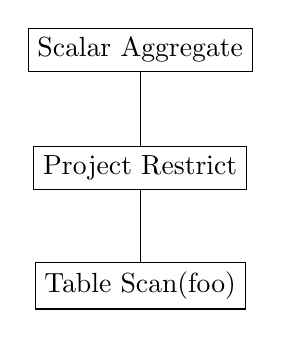
\begin{tikzpicture}[level/.style={sibling distance=60mm/#1}]
\node[rectangle,draw] (z){Scalar Aggregate}
		child { node[rectangle,draw] (b) {Project Restrict}
			child { node[rectangle,draw] (c) {Table Scan(foo)} }
};
\end{tikzpicture}
\caption{Operation Tree for simple count(*) query}
\label{fig:countTree}
\end{figure}

This operation needs to be applied to all regions for the table. It can be performed sequentially--just scan all the rows and count them one by one. Unfortunately, this sequential scanning is very slow for large data sets--we'd like to parallelize it as much as possible.

An alternative is to use a two-stage processing algorithm similar to MapReduce. In this situation, we know that we have multiple independent units of data--specifically, HBase regions. We can compute a separate intermediate count for each region in parallel, and then sum all the intermediate counts sequentially in order to generate our final count.

Now consider a slighty more complex example. Suppose that we are executing the sql
\begin{lstlisting}[frame=single,captionpos=b,caption=Aggregate over join,language=SQL]
select 
	count(*) 
from 
		foo f,
		bar b
where f.foo = b.foo
\end{lstlisting}
This query plan breaks down to the Operation Tree seen in figure \ref{fig:countOverJoinTree}.

\begin{figure}
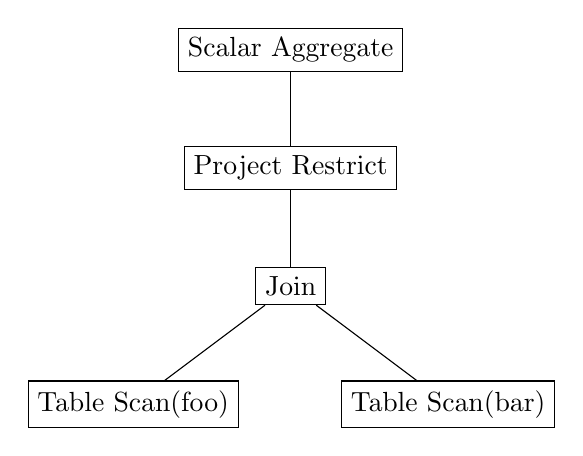
\begin{tikzpicture}[level/.style={sibling distance=120mm/#1}]
\node[rectangle,draw] (z){Scalar Aggregate}
		child { node[rectangle,draw] (b) {Project Restrict}
		child { node[rectangle,draw] (c) {Join}
			child { node[rectangle,draw] (d) {Table Scan(foo)} }
			child { node[rectangle,draw] (e) {Table Scan(bar)} }
	}
};
\end{tikzpicture}
\caption{Operation Tree for Aggregating over a Join}
\label{fig:countOverJoinTree}
\end{figure}

This is harder to imagine an efficient parallelization. Suppose that we could manage to parallelize the join\footnote{Which we can using Merge Sort Join}. In this case it makes more sense to do three stages

\begin{enumerate}
\item Join tables, placing output into intermediate storage
\item generate intermediate counts for joined values
\item merge intermediate counts to generate final results.
\end{enumerate}

This roughly encapsulates the main structure for parallelization in SpliceMachine

\subsection{Splitting Operations}
Given a SQL statement, we always compute an Operation tree that performs our pysical operations, so it's more convenient to discuss operation trees directly than it is to talk about SQL statements themselves.

We define an \emph{operation} as a node within an operation tree. An operation is either \emph{parallel} or \emph{sequential}. A Sequential operation is \emph{not} amenable to parallel execution--it will always be performed sequentially over rows one row at a time.

A Parallel operation, by contrast, is designed to execute in two stages: a \emph{parallel}\footnote{sometimes also referred to as a \emph{sink}} phase, and a \emph{sequential}\footnote{sometimes referred to as a \emph{scan}} phase. 

The parallel phase is strictly confined. During the parallel phase, the operation can take in rows from operations below it, and the output of the operation is written directly to storage\footnote{usually temporary storage, but it's not always required}. 

After all tasks involved in the parallel phase complete, the sequential phase begins (assuming that the operation has a sequential phase).

Thus, we can consider an operation tree as a tree of Sequential and Parallel operations. To correctly execute this tree, we perform a depth-first execution of parallel stages. Each parallel phase encompasses all sequential operations between the parallel operation and the previous parallel operation (or the bottommost operation on the tree). All parallel operations which are lower on the tree \emph{must} complete their parallel phases before the next lowest parallel operation can begin.

So, considering the join example as in Figure \ref{fig:countOverJoinTree}, we see that we have two parallel operations: the Join operation and the Scalar Aggregate. To execute this, we first execute the Join's parallel phase. We thus proceed in a depth-first manner. Since the Join is below the Scalar Aggregate, we execute the Join's parallel operation, writing its intermediate output to a temporary space. This is equivalent to a tree as in Figure \ref{fig:parallelJoinTree}

\begin{figure}
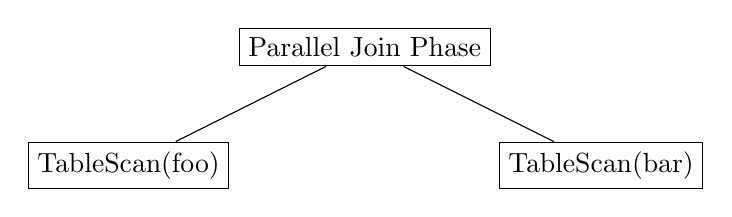
\begin{tikzpicture}[level/.style={sibling distance=60mm/#1}]
\node[rectangle,draw](z){Parallel Join Phase}
	child {node[rectangle,draw](a) {TableScan(foo)}}
	child {node[rectangle,draw](b) {TableScan(bar)}}
;
\end{tikzpicture}
\caption{Operation Tree for a Parallel Join}
\label{fig:parallelJoinTree}
\end{figure}

We execute this tree in parallel, one instance for each Task that we submit. The output of this tree is written into intermediate storage, and then we proceed to the next tree to execute, as in Figure \ref{fig:parallelAggOverJoin}.

\begin{figure}
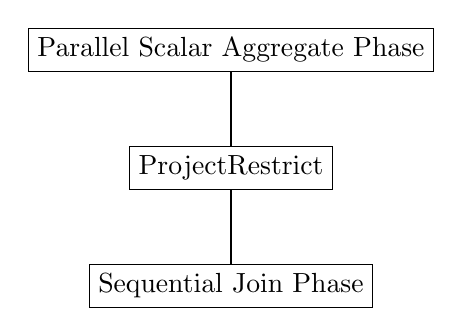
\begin{tikzpicture}[level/.style={sibling distance=60mm/#1}]
\node[rectangle,draw](z){Parallel Scalar Aggregate Phase}
	child {node[rectangle,draw](a) {ProjectRestrict}
	child {node[rectangle,draw](b) {Sequential Join Phase} }
}
;
\end{tikzpicture}
\label{fig:parallelAggOverJoin}
\caption{Operation Tree for Aggregate over Join}
\end{figure}

We can repeat this procedure for arbitrarily complex operation trees (and hence arbitrarily complex SQL statements), and it allows us to execute operations using massive parallelization, while still generating correct sequential results in the end.

\section{TEMP Space}
In order to execute operation trees in the manner we just described, we must have a location where we can store intermediate results. In SpliceMachine\footnote{as ov v0.5. Future versions may eliminate or change this} we use an HBase table called \temp as our intermediate storage.

\temp is an HBase table like any other, which retains data in sorted order, with a few specific modifications.

First, \temp has a different compaction strategy than other tables. Because data is made to exist in \temp for only the length of time taken to perform the next query(or return results to the client), we have no need to compact this data into new files for future IO. As a consequence, when compaction occurs, we only retain store files which contain data for queries which are currently active--all other data is ignored. This leads to hyper-efficient compactions.

Secondly, and far more importantly, \temp is split into $N$ buckets\footnote{The current implementation is to have $N=16$, but future implementations will likely make this more flexible}. These buckets allow some operations to keep data in sorted order without incurring the performance penalty of inserting into a sorted table.

\section{Operation Implementations}
This section describes the various algorithms chosen for the major operations.

\subsection{Parallel Operations over non-scan queries}
All parallel operations require that there be a scan to execute before they can submit tasks (and thus actually be parallel). If the underlying data structure does not have a relevant HBase table (e.g. a values() clause), then the parallel task will become sequential over the in-memory representation.

\subsection{Table Scans}
Table scans are the most fundamental operation in SpliceMachine--nearly all operations require a table scan at one point or another. Its purpose is simple--to scan data in a transactional manner, and to apply any predicates at the lowest possible level.

The basic implementation is sequential: data is scanned in the sort order of the table. As rows are visited, predicates are applied to determine whether or not this row should be included in the output.

For our purposes, a \emph{predicate} is a clause in a query which limits the amount of data which is returned. For example, $a=10$ is a predicate.

When a table is sorted, and a predicate is applied to the sort key \emph{in order}, then the table scan will bound the underlying HBase scan so that fewer rows will be visited. 

\begin{exmp}[Bounding a TableScan with a sort predicate]
Suppose $T$ is a table with columns $(a,b,c,d)$, and primary key $(b,a)$. Then, consider the SQL

\begin{lstlisting}[frame=single,captionpos=b,caption=SQL for bounded scan,language=SQL]
	select * from T where b = 10 
\end{lstlisting}

				This SQL will construct a table scan which is bounded so that only rows which have keys in the range $[10,11)$ are considered.

				By contrast, the sql

\begin{lstlisting}[frame=single,captionpos=b,caption=SQL for unbounded scan,language=SQL]
	select * from T where a = 10 
\end{lstlisting}
				will not be able to bound the rows--it must interact with every row in $T$ to determine the correct result
\end{exmp}

Predicates are applied at the byte level--data is \emph{not} decoded in order to check predicates. Instead, values are encoded into byte arrays, and the comparison is performed using lexicographic sort order\footnote{This is the primary reason why data is encoded in sorted order}.

It is important to note that (as of v0.5) Table scans are \emph{not} parallel operations. While the application of predicates \emph{could} be parallelized, Table scans are assumed to be short(in which case it is more efficient to perform a sequential scan), bounded by a sort order(either a primary key or an index), or underneath a parallel operation. In any of these three cases, a parallel Table scan operation would pose a performance penalty. However, this does mean that full table scans which are not under another parallel operation will take time linear in the number of rows. 

\subsubsection{Multi-probe scans}
When a table is sorted via a primary key or index, and the keyed columns are used in a SQL \emph{in} clause (where a key is allowed to match one of several values), then the table scan may produce a \emph{Multi-probe Scan}.

A Multi-probe scan is a table scan which has multiple separate bounding scans. Thus, it is possible to create multiple scans, each only responsible for scanning data which matches one entry in the clause.

\begin{exmp}[Multiple Bounds on a table scan]
Suppose $T$ is a table with columns $(a,b,c,d)$, and a primary key $(b,a)$. Then, consider the SQL

\begin{lstlisting}[frame=single,captionpos=b,caption=SQL for multiple bounds,language=SQL]
	select * from T where b in (10,15) and a = 5
\end{lstlisting}
Then the table scan is a multi-probe scan with two scans: $[10,11)$ and $[15,16)$, each of which will apply the $a=5$ predicate.
\end{exmp}

This technique can be used with an arbitrarily large number of entries in the \emph{in} clause. Be aware, however, that this may result in a massive increase in the number of tasks that need to be executed for parallel scans, which may incur a performance penalty.

\subsection{Index lookups}
Indices typically do not contain all the columns in a table\footnote{When they do, they are referred to as \emph{covering indices}}, so in order to fill some queries, an index lookup must be performed.

Index lookups in SpliceMachine are exceptionally expensive, because each request must go across the network to another table (potentially another server).

To avoid the network cost for every row, SpliceMachine batches up index lookups, and performs an HBase \emph{multi-get} to fetch multiple rows in bulk. To further reduce latency, SpliceMachine also performs \emph{forward fetches}--it uses a background thread to fetch the next batch of rows before it is requested.

Index lookup operations are usually referred to by their Derby reference, as \emph{IndexRowToBaseRow} or just \emph{IndexRow} operations; they are all sequential operations, designed to fit within a larger operation tree.

\subsection{ProjectRestrict}
There are two forms of operations which are done to transform and limit data in ways which are not amenable to raw table scans.

One operation is referred to as a \emph{projection}. Projections are transformations of the data, such as dividing two numbers, or computing substrings, etc. 

Another operation is referred to as a \emph{restriction}. Restrictions are mechanisms for filtering out rows which do not match predicate, but whose predicate is too complex to be converted into a scan qualifier.

In SpliceMachine, These two tasks are constructed in a single \emph{ProjectRestrict} operation. ProjectRestrict operations are sequential, and operate against a single row at a time.

\subsection{Aggregation}
Aggregation is a central theme of many SQL queries. In SpliceMachine, aggregation comes in four major forms:

\begin{description}
				\item[Scalar Aggregates] take in many rows, and output exactly one result.
				\item[Grouped Aggregates] emit one row per \emph{grouping key}
				\item[Distinct Scalar Aggregates] remove duplicate rows, then perform a scalar aggregate.
				\item[Distinct Grouped Aggregates] remove duplicate entries, then perform a grouped aggregate.
\end{description}
\subsubsection{Scalar Aggregates}
Scalar aggregation is a parallel operation, which aggregates \emph{all} matching rows into a \emph{single} row value. 

The parallel phase of a scalar aggregation consists of reading all data from its subtree, and aggregating the result. When its subtree runs out of rows, the aggregated value is finalized and written into \temp. Then the sequential phase of the operation reads the intermediate counts out and merges them together to form a final result.

\subsubsection{Grouped}
Grouped Aggregation is a parallel operation, which aggregates rows around a set of \emph{grouping keys}. 

The parallel phase of the grouped aggregation consists of reading data from its subtree, and placing each row into a hashtable. If the grouping keys already exist in the hashtable, then the row will be merged together to form an aggregated count; if they are not, then the row is added. To avoid overusing memory, this hashtable is bounded; when the number of rows in the hashtable exceeds a threshold, then a row is evicted and written to \temp. The sequential phase will then read each row that is stored in \temp and merge together matching entries.

When the grouped aggregate is underneath another parallel operation, the sequential phase will occur in parallel; in these cases, we'll need to ensure that a single task will need to read all data for a specific key. To perform this, we use a \emph{Region-aware Scanner}. This scanner will read rows off of other regions as necessary to ensure that grouping keys will be treated by one and only one region.

\subsubsection{Distinct Grouped}
Distinct Grouped Aggregates are special cases of Grouped Aggregation, except that duplicate entries are discarded during the parallel phase, rather than aggregated.

Additionally, distinct grouped aggregates will overwrite rows in \temp, which avoid duplication across multiple regions.

\subsubsection{Distinct Scalar}
Distinct Scalar operations is a 2-phase parallel operation. The first phase is identical to a distinct grouped aggregate, while the second phase is equivalent to a scalar aggregation.

\subsection{Sorting}
Sorting is a very simple parallel operation, which writes data into \temp, using the sort keys as row keys, then reading data out of \temp.

Distinct sorting is a sort model that is similar to Distinct Grouped aggregation, but without the final merge step. In effect, it throws away duplicate entries, then scans the non-duplicated entries out of \temp.

\subsection{Distinct Scan}
Distinct scanning in SpliceMachine is functionally equivalent to Distinct sorting in SpliceMachine. The only reason it exists is that distinct scan does not \emph{require} sorting (although the implementation will sort in effect).

\subsection{Joins}
Joins come in several varieties, and are useful in different contexts.
\subsubsection{MergeSortJoin}
a MergeSort join is a parallel operation which is useful for performing joins against two large tables which are not sorted according to the join key.

The MergeSort Join algorithm is simple. In the parallel phase, the left and right sides of the table are scanned in parallel, and written to \temp. The row key in \temp are the join keys, plus a \emph{join ordinal}, which is a 1-byte entry determining which side of the join the row came from. This ordinal is such that right-side rows are sorted before left-side rows. Then, during the sequential phase, all right-side entries \emph{for a single join key} are read into memory. After this occurs, all left-side rows which match taht join key are read.

MergeSortJoin requires that only the right side rows \emph{for a given key} fit within memory\footnote{This does not mean that the right hand side must fit completely within memory, only that the rows needed to join to a single left-hand-side row do.}. This makes it effective when both tables to be joined are very large and are not sorted according to the join keys. If the right-hand-side is very small, then Broadcast joins are more effective; if the two tables are both sorted according to the join keys, then MergeJoin is more appropriate\footnote{In most cases. MergeJoin is not parallel, however, so some queries will not perform well when using straight MergeJoins}.

\subsubsection{MergeJoin}
MergeJoin is a sequential equivalent of MergeSortJoin, in that it reads data from two sorted locations; it is different in that it assumes that both the left and right side of the join are sorted in the same ordering. When this is satisfied, MergeJoin will open only two scans--one for the right side, and one for the left. It will then merge data together in sequence, just as in the classic MergeSort algorithm.

MergeJoin requires that both tables to be joined are sorted according to the join keys for the query, or else it cannot be used. Within this constraint, however, there is no limitation on the resources available to perform a MergeJoin.

As MergeJoin is \emph{not} a parallel operation, it may be desirable to prefer MergeSortJoin whenever there is high selectivity in the join (that is, that many rows will not match the given join criteria, so the output of the join is very small) and when there are no parallel operations on top of the MergeJoin itself. Otherwise, it is almost always preferable to use MergeJoins whenever possible, as it will avoid the extra cost of sinking data into \temp.

\subsubsection{Broadcast}
When the right side of a join is extremely small, it is cheaper to pay the penalty to just scan the entire table and then perform the join in memory--these situations form the basis of the Broadcast Join.

Broadcast Joins operate sequentially by first reading the \emph{entire} right-side into the left side's memory space. Then, for each row on the left side, it refers to its memory space for the proper right-side rows.

Broadcast Joins require that the entire right hand side be able to fit within the memory space of the left-hand-side's operating capacity. As there is an initial latency due to reading the right hand side, Broadcasts may perform more poorly than MergeJoins when the right side is large (even if the right side can fit within memory).

Broadcast Joins are \emph{not} parallel operations, so a broadcast join operation will not execute in parallel unless a parallel operation is above it.

\subsubsection{NestedLoopJoin}
NestedLoopJoins are the simplest form of join. It is a sequential operation that executes a join using a "nested loop"; for each left row that is scanned in, a new scan is created for the right side, with the matching qualifiers. A joined row is then created for each row emitted from the right-side scan. When that scan is exhausted, the left side is allowed to proceed to the next row and repeat.

NestedLoopJoins displays very poor performance in most cases, and should be avoided as much as possible. The only situation in which a NestedLoopJoin must be used is for non-equi-joins\footnote{As of v0.5. Future versions may modify Merge and MergeSort joins to perform non-equi-joins} in which the right hand side is considered too large to use a Broadcast join with.


\subsection{Unions}
Unions come in two forms: \emph{Union All} and \emph{Union}. A UnionAll operation will return \emph{all} the rows from the left side with \emph{all} the rows from the right side, while a Union operation will return only the distinct elements which are contained in either the left or the right side.

The query optimizer will rewrite a Union operation as a Distinct Sort over a UnionAll operation, so the only true implementation of Union is the UnionAll.

When a UnionAll is over a table scan, then it will emit all the left rows, then a separate region will emit all the right rows. When both left and right are wholly in memory (i.e. over a values clause), then UnionAll will emit all left then all right within the same java heap.

Since UnionAll is effectively two table scans in sequence, it is implemented as a sequential operation. As Union is effectively a distinct sort, Unions are parallel.

\subsection{DML Write operations}
DML write operations come in three flavors(Inserts, Updates, and Deletes), all of which follow the same basic pattern. Firstly, all DML write operations are parallel--when executed over a scan, they will perform that scan in parallel. However, when the underlying structure does not correspond to a scan (i.e. a values() clause), then the operation is performed sequentially over the in-memory representation.

Secondly, DML write operations do not write to \temp, instead they write to the destination table directly, and those writes are goverened by Snapshot Isolation. Thus, DML write operations may throw a Write/Write Conflict during concurrent access. 

\subsection{Insert}
Inserts are a very straightforward implementation, taking rows from the operation subtree and writing them to the destination table in bulk. If the destination table has a primary key, then Inserts will construct those. Similarly, if there is a sequential field, Inserts will generate the next sequential id for insertion.

\subsubsection{Sequential Column}
SpliceMachine supports (as of v0.5) a limited form of a sequential identifier. However, there are some notable differences between a SpliceMachine sequence and a more traditional sequence.

In a traditional (single-node) database, sequences are fairly trivial to implement-- a durable atomic counter is all that is necessary. However, creating a durable atomic counter which can be accessed by many nodes is a significant challenge, and often imposes a high degree of latency.

To avoid the increased latency\footnote{as of v0.5}, SpliceMachine uses a \emph{partially-ordered} implementation. In this implementation, there is a column on the HBase table $SPLICE\_SEQUENCES$ which is unique for each sequential column in the system. This column stores a long which contains the last \emph{reserved} sequence id.

When a node wishes to use the sequence, it will attempt to \emph{reserve} a block of sequence ids (by default, 1000). This requires a network call to update the column in $SPLICE\_SEQUENCES$. After this call, sequence ids are issued in order until the block is exhausted. When that occurs, the node will attempt to reserve another block, and so on.

Because multiple servers may be executing in parallel, this algorithm means that some rows may appear out of order, and not all sequence ids are guaranteed to occur. However, each sequence id \emph{is} unique, and thus may be used as a primary key (if needed). Note however that using a sequential field as a primary key will result in uneven write performance, as only a few regions at a time will accept writes.

\subsection{Updates}

Updates are a parallel operation which attempts to modify data in place. Under Snapshot Isolation, an Update is actually an insert with a new timestamp, so the functional structures are similar.

As of v0.5, Updates cannot be performed over a parallel suboperation, because the location of the row to be updated is lost during the suboperation's parallel execution phase.

\subsubsection{Updating Primary Keys}
When a primary key needs to be updated, its HBase row key must be changed. However, HBase does not allow the mutation of a row key directly. Instead, the Update operation must delete the old row and then insert the new one. In order to do this, Updates must be sure to acquire all relevant information with which to move the row; this may require a remote hbase GET operation to be performed.

When primary keys are not modified (or there are no primary keys on the table), then an update will behave exactly as if it were an insert.

\subsection{Deletes}
Deletes in SpliceMachines are specialized insertions--an empty byte array is written to the row location, and Snapshot Isolation appends a \emph{tombstone} value to the location, indicating that the row should be considered deleted.

As of v0.5, Deletes cannot be performed over a parallel suboperation, because the location of the row to be deleted is lost during the suboperation's parallel execution phase.

\subsection{Import}
Imports are a specialized procedure in SpliceMachine to efficiently load a large volume of data into the system relatively quickly. They are parallel \emph{in the number of files}--that is, each file to be imported will be granted its own task. 

Files must be stored in HDFS before they may be imported. This is because there is no way of knowing a priori which node will actually perform the import processing (tasks are assigned at random), and because if a task fails, it may be necessary to retry that task on a different node; therefore, the data file \emph{must} be equally accessible to all nodes in the same way, which requires HDFS\footnote{There is often some confusion here, so it is important to emphasize. There is \emph{absolutely no} way that a file stored on local storage of a single machine could be successfully imported except by that machine. If that machine fails, then the import must fail. SpliceMachine has opted for the design of fault tolerance in this case, which means allowing multiple machines access. HDFS is a non-negotiable part of this design. }.

Within a task, there is a single thread which reads data off of HDFS, and then multiple \emph{processor} threads, which take data from the reader thread, parse it into the proper binary representation, and attempt to write that representation to the destination table. In this way, an import is much like an Insert, but where an insert operation requires the underlying operation to be a table scan (and hence already in the proper storage format), Imports require data to be in a user-specified format.

\subsection{Subqueries}
Subqueries are typically implemented as a ProjectRestrict operation, where the ProjectionOperation is the execution of the subquery. This means that, while the subquery \emph{itself} may be a parallel operation, the \emph{full} query may not be.

\section{Appendix: List of Operations}
This appendix is a short list of operations, as well as some brief information about them (whether the operation is parallel or sequential, and what the row key is for \temp if the operation is parallel).

To make this table more concise, we introduce the variables described in Table \ref{tab:op-legend}.

\clearpage
\begin{table}
\begin{tabular}{|l|l|}
				\hline
				\bf{Variable}	&	\bf{Description}								\\	\hline
				$t$			&	Unique Task ID												\\	\hline
				$f$			&	Fixed bucket id												\\	\hline
				$o$			&	Unique Operation ID										\\	\hline
				$uuid$	&	Unique Row ID													\\	\hline
				$g$			& Grouped/Sorting columns								\\	\hline
				$j$			&	Join Ordinal(either left or right)		\\	\hline
				$b(g)$	& Unique bucket for the grouped columns	\\	\hline
\end{tabular}
\\
\caption{Variable definitions for Operation List}
\label{tab:op-legend}
\end{table}

\begin{table}
				\begin{tabular}{|l|c|p{6cm}|}
								\hline
								\bf{Operation}	&	\bf{Is Parallel?}	&	\bf{Output Row Key} \\ \hline

								TableScan													&	No	&	\\	\hline
								Index Lookup											&	No	&	\\	\hline
								ProjectRestrict										&	No	&	\\	\hline
								Union All													&	No	&	\\	\hline
								ScalarAggregate										&	Yes	&	$f|o|uuid|t$				\\	\hline
								GroupedAggregate									&	Yes	&	$b(g)|o|g|uuid|t$		\\	\hline
								DistinctGroupedAggregate					&	Yes	&	$b(g)|o|g$					\\	\hline
								Sort															&	Yes	&	$f|o|g|uuid|t$			\\	\hline
								Distinct Sort											&	Yes	&	$f|o|g$							\\	\hline
								MergeSortJoin											&	Yes	&	$b(g)|o|g|j|uuid|t$	\\	\hline
								DistinctScalarAggregate(Phase 1)	&	Yes	&	$b(g)|o|g$					\\	\hline
								DistinctScalarAggregate(Phase 2)	&	Yes	&	$f|o|uuid|t$				\\	\hline
								Union\tablefootnote{Unions are equivalent to Sort over a Union All}	&	Yes	&	$f|o|g|uuid|t$			\\	\hline
								MergeJoin													&	No	&	\\	\hline
								BroadcastJoin											&	No	&	\\	\hline
								Insert														&	Yes	&	table dependent \\ \hline
								Update														&	Yes	&	table dependent	\\	\hline
								Delete														&	Yes	&	table dependent	\\	\hline
								Import														&	Yes	&	table dependent \\ \hline
				\end{tabular}
				\caption{List Of Operations}
				\label{table:op-list}
\end{table}

%End Operation Execution Chapter

\endgroup

\end{document}
